%{{\chapter{An Introduction to Partial Differential Equations and Diffusion in Biological Settings}}}
{{\chapter{Uma introdução às equações diferenciais parciais e difusão em configurações biológicas}}}

\begin{citacao}
%{{I do not know what I may appear to the world; but to myself I seem to have been only like a boy playing on the seashore, and diverting myself in now and then finding a smoother pebble or prettier shellthan ordinary, whilst the great ocean of truth lay all undiscovered before me.}}
{{Não sei o que posso parecer ao mundo; mas para mim mesmo pareço ter sido apenas como um menino brincando na praia, e me divertindo de vez em quando, encontrando um seixo mais liso ou uma concha mais bonita do que o comum, enquanto o grande oceano da verdade estava todo escondido diante de mim.}}

Isacc Newton (1642-1727) p 90 E. T. Bell (1937) Men of Mathematics Simon \& Schuster, N.Y.
\end{citacao}

%{{Part of our admiration for nature stems from the fact that it continually surprises us with its infinite variation, regardless of the scale of observation. This holds true of microscopic worlds; the surface of a cell for example, consistsof myriad buoyant macromolecules distributed haphazardly in a viscous lipid sea. On the broad scale, that of continents or ecosystems, the fabric of habitats is like a patchwork quilt with a wide variety of local conditions,somefavoring one species, some favoring another.}}
{{Parte da nossa admiração pela natureza advém do fato de ela nos surpreender continuamente com sua variação infinita, independente da escala de observação. Isso é verdade para mundos microscópicos; a superfície de uma célula, por exemplo, consiste em uma miríade de flutuantes macromoléculas distribuídas ao acaso em um mar viscoso de lipídios. Em larga escala, a de continentes ou ecossistemas, o tecido dos habitats é como uma colcha de retalhos com uma grande variedade de condições locais, algumas favorecendo uma espécie, outras favorecendo outra.}}

%{{For this reason, real natural systems behave in a way that reflects an underlying spatial variation. Despite our idealizations, no speciesactually consists of identical individuals, since not all individuals are equally exposed to a constant environment. Similarly, on the molecular level, rarelydoreactions take place in a homogeneous soup of chemicals. Somehow the effect of spatial organization does influence the way individual particles or molecules interact.}}
{{Por esse motivo, os sistemas naturais reais se comportam de uma maneira que reflete uma variação espacial subjacente. Apesar de nossas idealizações, nenhuma espécie realmente consiste em indivíduos idênticos, uma vez que nem todos os indivíduos estão igualmente expostos a um ambiente constante. Da mesma forma, no nível molecular, raramente as reações ocorrem em uma sopa homogênea de produtos químicos. De alguma forma, o efeito da organização espacial influencia a maneira como as partículas ou moléculas individuais interagem.}}

%{{In the three chapters to follow, our purposeis to expose how spatial variation influences the motion, distribution, and persistence of species. We shall see that in the fine balance that exists between interdependent species, the spatial diversity of the system can have subtle but important effects. Conversely, the interactions of unlike species can result in spatial heterogeneityand lead to the appearance of patterns out of a uniform state. Our initial goal is to introduce the concepts underlying spatially dependent processes and the partial differential equations(PDEs)that describe these. The discussion is somewhatgeneral,with examples drawn from molecular, cellular, and population levels. Later we will apply the ideas to more specific cases with the aim of gaining an understanding of phenomena.}}
{{Nos três capítulos a seguir, nosso objetivo é expor como a variação espacial influencia o movimento, a distribuição e a persistência das espécies. Veremos que, no equilíbrio tênue que existe entre as espécies interdependentes, a diversidade espacial do sistema pode ter efeitos sutis, mas importantes. Por outro lado, as interações de espécies diferentes podem resultar em heterogeneidade espacial e levar ao aparecimento de padrões fora de um estado uniforme. Nosso objetivo inicial é apresentar os conceitos subjacentes aos processos dependentes do espaço e às equações diferenciais parciais (PDEs) que os descrevem. A discussão é um tanto geral, com exemplos extraídos de níveis moleculares, celulares e populacionais. Posteriormente, aplicaremos as ideias a casos mais específicos com o objetivo de obter uma compreensão dos fenômenos.}}

%{{In this chapter we discover primarily how partial differential equations arise and by what procedures they can be assembled into statementsthat are reasonable mathematically as well as physically.We see that under appropriate assumptions the motion of groupsof particles (whether molecules, cells, or organisms) can be represented by statements of mass or particle conservation that involve partial derivatives.}}
{{Neste capítulo, descobrimos principalmente como as equações diferenciais parciais surgem e por quais procedimentos elas podem ser reunidas em afirmações que são razoáveis tanto matematicamente quanto fisicamente. Vemos que, sob suposições apropriadas, o movimento de grupos de partículas (sejam moléculas, células ou organismos) pode ser representado por declarações de conservação de massa ou partícula que envolvem derivadas parciais.}}

%{{Such statements, often called conservation or balance equations, are universal in mathematical descriptions of the natural sciences. Indeed practically every PDE that depicts a physical process is ultimately based on principles of conservation----of matter, momentum, or energy.}}
{{Essas afirmações, frequentemente chamadas de equações de conservação ou equilíbrio, são universais nas descrições matemáticas das ciências naturais. Na verdade, praticamente todo PDE que representa um processo físico é, em última análise, baseado em princípios de conservação - da matéria, quantidade de movimento ou energia.}}

%{{Before undertaking the derivation of balance equations, we devote Section 9.1 to a review of the material that forms much of the structural underpinning of the mathematical framework. Students well versed in advanced calculus may skim through this section. One of the key observationswe make is that the spatial variation in a distribution can lead to directional information. This proves conceptually useful in later discussions.}}
{{Antes de empreender a derivação das equações de equilíbrio, devotamos a Seção 9.1 a uma revisão do material que forma muito da base estrutural da estrutura matemática. Alunos bem versados em cálculo avançado podem folhear esta seção. Uma das principais observações que fazemos é que a variação espacial em uma distribuição pode levar a informações direcionais. Isso se prova conceitualmente útil em discussões posteriores.}}

%{{With this preparation wethen proceed with the derivation of statementsof conservation. This is accomplished in two stages. First, a simpleargument for one-dimensional settings is given in Section 9.2. This is followed by more rigorous derivations and a generalization to other geometries and higher dimensions. We then consider several specific phenomena --- including convection, diffusion, and attraction --- thraet sult in the motion of particles. Each phenomenon leads to special cases of the conservation equation. Such equations are derived in Section 9.4 and explored more fully later.}}
{{Com essa preparação, procedemos com a derivação das declarações de conservação. Isso é realizado em duas etapas. Primeiro, um argumento simples para configurações unidimensionais é fornecido na Seção 9.2. Isso é seguido por derivações mais rigorosas e uma generalização para outras geometrias e dimensões superiores. Em seguida, consideramos vários fenômenos específicos - incluindo convecção, difusão e atração - como resultado do movimento das partículas. Cada fenômeno leva a casos especiais da equação de conservação. Essas equações são derivadas na Seção 9.4 e exploradas com mais detalhes posteriormente.}}

%{{One example of applying such ideas to a universal process --- that of diffusion --- is illustrated in Sections 9.5 to 9.9. Derivation of the equation governing diffusion is rather straightforward if one accepts an assumptionknown as Fick's law. A more fundamental approach based on random-walk models is rather more sophisticated. Okubo (1980) and references therein should be consulted for finer details.}}
{{Um exemplo de aplicação de tais ideias a um processo universal --- o de difusão --- é ilustrado nas Seções 9.5 a 9.9. A derivação da equação que governa a difusão é bastante direta se aceitarmos uma suposição conhecida como lei de Fick. Uma abordagem mais fundamental baseada em modelos de passeio aleatório é um pouco mais sofisticada. Okubo (1980) e suas referências devem ser consultadas para maiores detalhes.}}

%{{Less straightforward is the process of actually solving the diffusion equation (or any other) PDE. Exploring the host of powerful techniques commonly applied by mathematicians in analyzing PDEs is beyond our scope. However, even before attempting to find a full solution, the form of the equation leads to an appreciation for the role of diffusion as a biological transport mechanism. A ubiquitous and metabolically free processonthe subcellular level, diffusion proves inefficient or totally useless on somewhat larger distance scales. Someof these observations and their implications are presentedin Sections 9.5 to 9.7.}}
{{Menos direto é o processo de realmente resolver a equação de difusão (ou qualquer outra) PDE. Explorar a série de técnicas poderosas comumente aplicadas por matemáticos na análise de PDEs está além do nosso escopo. No entanto, antes mesmo de tentar encontrar uma solução completa, a forma da equação leva a uma apreciação do papel da difusão como mecanismo de transporte biológico. Um processo ubíquo e metabolicamente livre no nível subcelular, a difusão se mostra ineficiente ou totalmente inútil em escalas de distância um tanto maiores. Algumas dessas observações e suas implicações são apresentadas nas Seções 9.5 a 9.7.}}

%{{Section 9.8 and the Appendix give some guidance on ways of solving the diffusion equation. We limit ourselves to separation of variables, a technique that is readily applied given a familiarity with ordinary differential equations(ODEs). Several basic solutions are derived, and others are given without formal justification in order to circumvent a lengthy mathematical excursion into the relevant techniques Section9.9describesan application of the diffusion equation to bioassay for mutation-inducing substances.}}
{{A Seção 9.8 e o Apêndice fornecem algumas orientações sobre as maneiras de resolver a equação de difusão. Nós nos limitamos à separação de variáveis, uma técnica que é prontamente aplicada devido à familiaridade com as equações diferenciais ordinárias (EDOs). Diversas soluções básicas são derivadas e outras são fornecidas sem justificativa formal, a fim de contornar uma longa excursão matemática nas técnicas relevantes. A Seção 9.9 descreve uma aplicação da equação de difusão a bioensaios para substâncias indutoras de mutação.}}

%{{For a rapid coverage of the key ideas in this chapter, the followingsequenceis recommended: Section 9.1 should be included or covered briefly in the interests of review. Sections 9.2 and 9.4 are essential for later material. Sections 9.3 and 9.5 can be assigned as independent reading or further research. Some highlights of the material in Section 9.8 or in the Appendix should be given, with particular emphasis on the role of boundary conditions in solutions of the diffusion equation. Familiarity with the examples may prove helpful but is not essential for mastering the material in Chapter 11.}}
{{Para uma cobertura rápida das ideias-chave deste capítulo, recomenda-se a seguinte sequência: A Seção 9.1 deve ser incluída ou abordada resumidamente para fins de revisão. As seções 9.2 e 9.4 são essenciais para materiais posteriores. As seções 9.3 e 9.5 podem ser atribuídas como leituras independentes ou pesquisas adicionais. Alguns destaques do material na Seção 9.8 ou no Apêndice devem ser dados, com ênfase particular no papel das condições de contorno nas soluções da equação de difusão. Familiaridade com os exemplos pode ser útil, mas não é essencial para o domínio do material do Capítulo 11.}}


%{{\section{FUNCTIONS OF SEVERAL VARIABLES: A REVIEW}}}

{{\section{FUNÇÕES DE DIVERSAS VARIÁVEIS: UMA REVISÃO}}}


%{{We begin this chapter by briefly reviewing the theory of functions of several variables with emphasis on the geometric concepts behind the mathematical ideas.}}
{{Começamos este capítulo revisando brevemente a teoria das funções de várias variáveis, com ênfase nos conceitos geométricos por trás das ideias matemáticas.}}


%{{Those of you who have had advanced calculus can skim quickly through this section or go directly to the next one.}}
Aqueles de vocês que tiveram cálculo avançado pode percorrer rapidamente nesta seção ou vá diretamente para a próxima.


\begin{comment}
First consider a real-valued function of two variables $x$ and $y$. In this chapter $x$ and $y$ will symbolize spatial coordinates of a point $(x, y)$, and
\begin{equation} z = f(x,y), \end{equation}
die value assigned to $(x, y)$ by the function/, will generally represent some spatially distributed quantity. Examples include
\end{comment}
%\begin{comment}
Considere primeiro uma função de valor real de duas variáveis $x$ e $y$. Neste capítulo, $x$ e $y$ simbolizam as coordenadas espaciais de um ponto $(x, y)$, e
\begin{equation} z = f(x,y), \end{equation}
o valor atribuído a $(x, y)$ pela função /, geralmente representa alguns quantidade espacialmente distribuída. Exemplos incluem
%\end{comment}

\begin{comment}
\begin{enumerate}
\item The density of a population at $(x, y)$.
\item The concentrationof a substance at $(x, y)$.
\item The temperature at $(x, y)$
\end{enumerate}
\end{comment}
%\begin{comment}
\begin{enumerate}
\item A densidade de uma população em $(x, y)$.
\item A concentração de uma substância em $(x, y)$.
\item A temperatura em $(x, y)$.
\end{enumerate}
%\end{comment}


\begin{comment}
A graph of the function $f$ is the set of points $(x, y, f(x, y)) \in \mathbb{R}^3$. The value $z = f(x, y)$ can be visualized as the height [assigned by the function $f$ to each point in the plane, $(x, y)$]. Equation (1) thus describes a surface, as shown in Figure 9.1(a).

Similarly, a function of three variables
$z = g(x, y, w)$ (2)
has a graph consisting of all points $(x, y, w, g(x, y, w))$. This is not as easy to draw, but the idea is analogous. (Every point in space is assigned a value by the function.)
\end{comment}
%\begin{comment}
Um gráfico da função $f$ é o conjunto de pontos $(x, y, f(x, y)) \in \mathbb {R}^3$. O valor $z = f(x, y)$ pode ser visualizado como a altura [atribuída pela função $ f $ a cada ponto no plano, $(x, y)$]. A equação (1) descreve uma superfície, como mostrado na Figura 9.1 (a).

Da mesma forma, uma função de três variáveis
$z = g (x, y, w)$ (2)
tem um gráfico que consiste em todos os pontos $(x, y, w, g (x, y, w))$. Não é tão fácil de desenhar, mas a ideia é análoga. (Cada ponto no espaço é atribuído um valor pela função.)
%\end{comment}


\begin{comment}
\end{comment}
%\begin{comment}

%\end{comment}

\begin{comment}
\end{comment}
%\begin{comment}

%\end{comment}

\begin{comment}
Sometimes it is more convenient to depict functions in other ways, some of which are shown in Figure 9.1 for functions of two and three variables. It is common to represent the behavior of a function of two variables by a set of contours for which
    $$f(x, y) = \mbox{constant}. (3)$$
    
In R2 these are called level curves and are simply loci for which a constant concentration or a constant density (or height) is maintained. As we shall see, they play an important role in me geometry of gradients and gradient fields.
\end{comment}
%\begin{comment}
Às vezes, é mais conveniente representar as funções de outras maneiras, algumas das quais são mostradas na Figura 9.1 para funções de duas ou três variáveis. É comum representar o comportamento de uma função de duas variáveis por um conjunto de contornos para os quais
\begin{equation}
f(x, y) = \mbox{constante}.
\end{equation}
    
Em $\mathbb{R}^{2}$, eles são chamados de curvas de nível e são simplesmente locais para os quais uma concentração constante ou uma densidade (ou altura) constante é mantida. Como veremos, eles desempenham um papel importante na geometria de gradientes e campos de gradiente.
%\end{comment}

\noindent
\begin{figure}[!ht]
\caption{As funções de duas ou três variáveis podem ser representadas graficamente de várias maneiras como:}
\begin{subfigure}[t]{0.33\linewidth}\centering
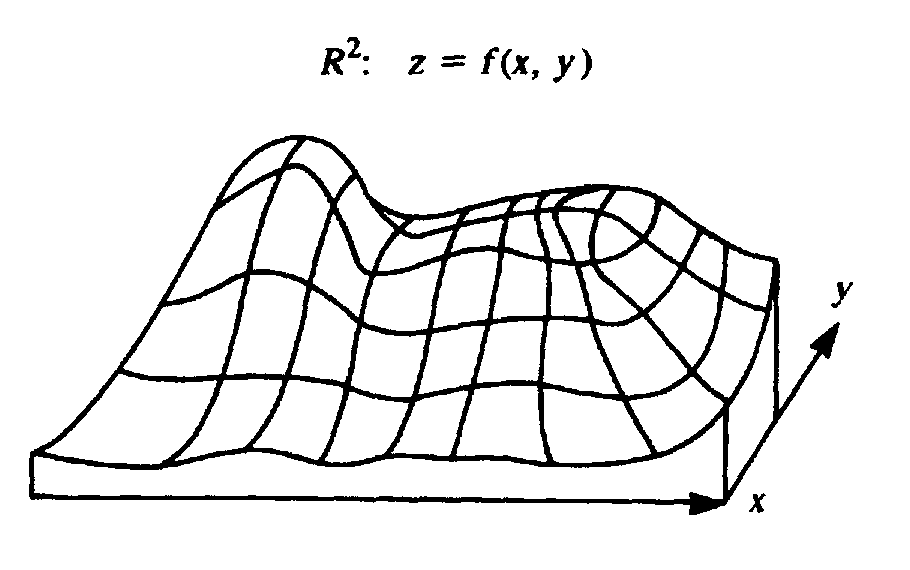
\includegraphics[scale=0.3]{figs/leah/fig09.01a.png}
\caption{\small uma superfície (apenas duas variáveis)}
\label{fig:09.01a}
\end{subfigure}
\begin{subfigure}[t]{0.33\linewidth}\centering
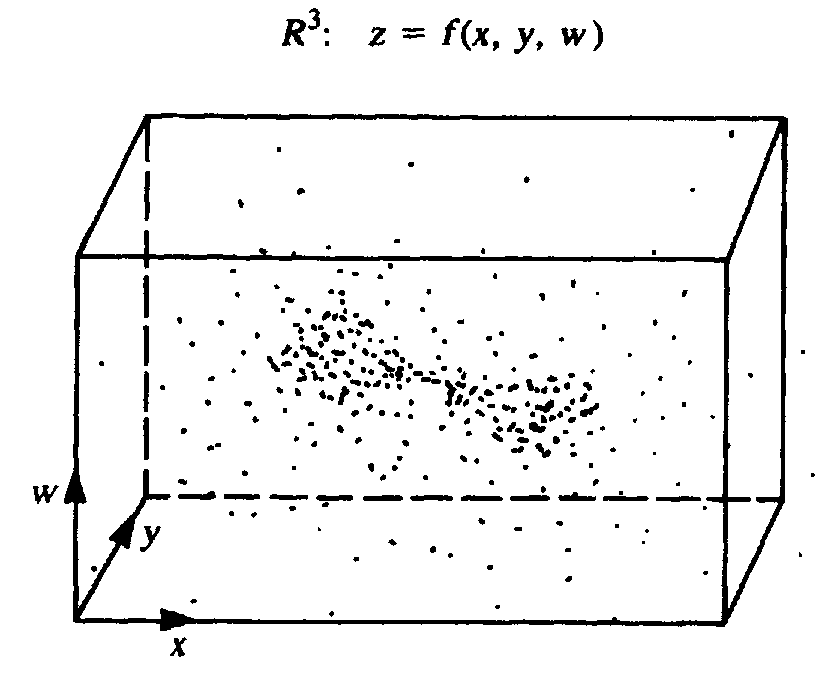
\includegraphics[scale=0.3]{figs/leah/fig09.01b.png}
\caption{\small uma distribuição de densidade no R3}
\label{fig:09.01b}
\end{subfigure}
\begin{subfigure}[t]{0.32\linewidth}\centering
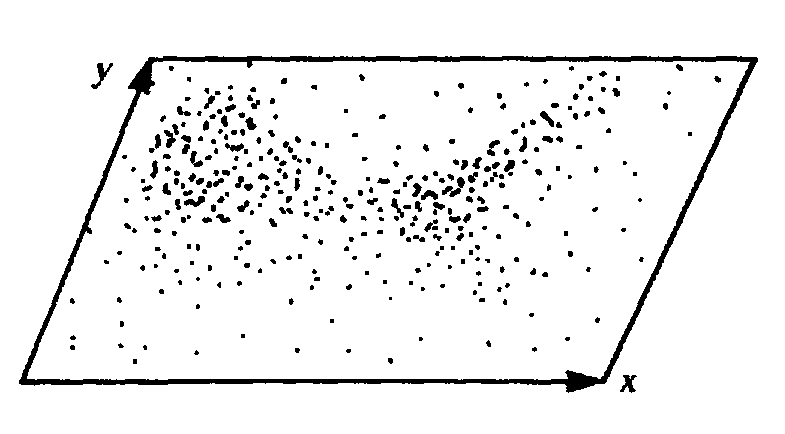
\includegraphics[scale=0.3]{figs/leah/fig09.01c.png}
\caption{\small uma distribuição de densidade no R2}
\label{fig:09.01c}
\end{subfigure}
\vfil
\begin{subfigure}[t]{0.5\linewidth}\centering
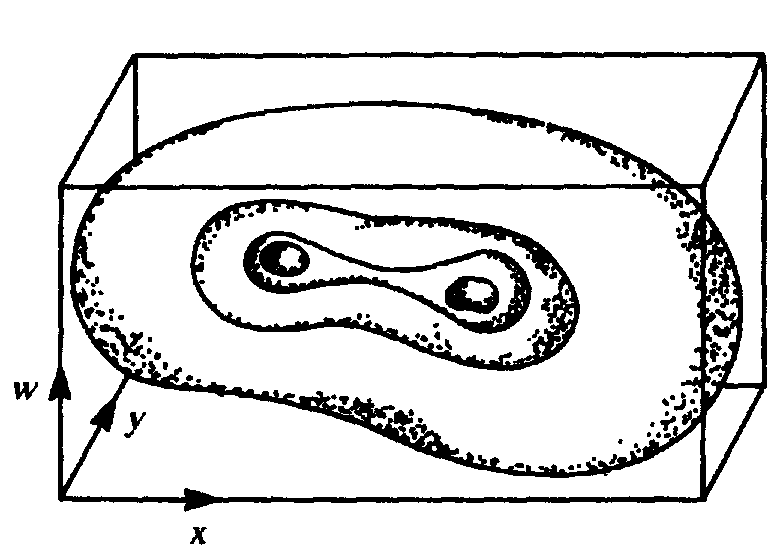
\includegraphics[scale=0.3]{figs/leah/fig09.01d.png}
\caption{\small superfície de nível}
\label{fig:09.01d}
\end{subfigure}
\begin{subfigure}[t]{0.5\linewidth}\centering
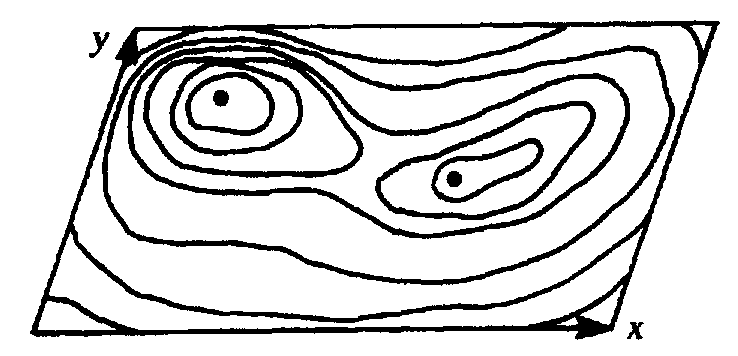
\includegraphics[scale=0.3]{figs/leah/fig09.01e.png}
\caption{\small curvas de nível}
\label{fig:09.01e}
\end{subfigure}
\end{figure}



\begin{comment}
In R3 the function of three variables given by (2) can similarly be represented by sets of points for which f(x, y, w) = constant. (4)
\end{comment}
%\begin{comment}
Em R3, a função de três variáveis dadas por (2) pode ser representada de forma semelhante por conjuntos de pontos para os quais
\begin{equation}\label{eq:09.04}
f(x, y, w) = \mathrm{constante}.
\end{equation}
%\end{comment}

\begin{comment}
Such loci area generalized version of level curves, but for obvious reasons these are called level surfaces [see Figure 9.1(d)]. To clarify with an example, consider a temperature field in three dimensions. The equitherms are then surfaces at which some given constant temperature is maintained. If heat sources are located at two points, the resulting equithermal surfacesmight look something like those shown in Figure 9.1(d).
\end{comment}
%\begin{comment}
Esses loci são uma versão generalizada das curvas de nível, mas por razões óbvias são chamadas de superfícies de nível [ver Figura 9.1 (d)]. Para esclarecer com um exemplo, considere um campo de temperatura em três dimensões. Os equitérmos são, então, superfícies nas quais uma dada temperatura constante é mantida. Se as fontes de calor estiverem localizadas em dois pontos, as superfícies equitérmicas resultantes podem se parecer com as mostradas na Figura 9.1 (d).
%\end{comment}


\begin{comment}
In the context of this chapter, level curves or surfaces might represent the loci on which (1) population density is constant or (2) chemical concentration is constant.

We shall be concerned primarily with statements about how spatial distributionschange with time; frequently it will be clear that the movement of one substance or population is closely linked to the distribution of another.

Consider the following simple example.An organism crawling on a flat surface may adapt its motion to the search for food particles. Imagine then that the dots in Figure 9.1(c) represent nutrient particle concentration. The observed path should ideally lead to the site of greatest concentration. To sense an increase in the ambient concentration level, an organism must continually cross level curves of the particle distribution. Per unit distance traveled, this crossing can be done most efficientlyby maintaining a path orthogonal to the level curves;in other words, a tangent vector to the path should be perpendicular to a tangent to a level curve through a given point. This assertion can be verified using rather elementary calculus of several variables. It can alsobe shown that the destination will be a critical point of the function (in this case a local maximum) but not necessarily the global maximum.
\end{comment}
%\begin{comment}
No contexto deste capítulo, curvas de nível ou superfícies podem representar os loci nos quais (1) a densidade populacional é constante ou (2) a concentração química é constante.

Estaremos preocupados principalmente com afirmações sobre como as distribuições espaciais mudam com o tempo; frequentemente ficará claro que o movimento de uma substância ou população está intimamente ligado à distribuição de outra.

Considere o seguinte exemplo simples. Um organismo rastejando sobre uma superfície plana pode adaptar seu movimento à procura de partículas de alimento. Imagine então que os pontos na Figura 9.1 (c) representam a concentração de partículas de nutrientes. O caminho observado deve, idealmente, levar ao local de maior concentração. Para sentir um aumento no nível de concentração ambiente, um organismo deve cruzar continuamente as curvas de nível da distribuição de partículas. Por unidade de distância percorrida, esse cruzamento pode ser feito de forma mais eficiente, mantendo um caminho ortogonal às curvas de nível; em outras palavras, um vetor tangente ao caminho deve ser perpendicular a uma tangente a uma curva de nível através de um determinado ponto. Esta afirmação pode ser verificada usando cálculos bastante elementares de várias variáveis. Também pode ser mostrado que o destino será um ponto crítico da função (neste caso, um máximo local), mas não necessariamente o máximo global.
%\end{comment}


\begin{comment}
In calculus a common place analogy is often drawn in explaining these ideas. Hikers often use topographical maps which are two-dimensional representations of the height of the terrain. The curves on such maps are level curves for the function f(x, y) = height above sea level at latitude x and longitude y. Mountain peaks, valleys, and mountain passes are critical points off(x, y) that correspond to local maxima, minima, and saddle points respectively. Using local information only (for example, walking uphill with no information other than the local slope), one can attain a local maximum, but this may or may not be the highest possible peak.
\end{comment}
%\begin{comment}
No cálculo, uma analogia comum é frequentemente desenhada para explicar essas ideias. Os caminhantes costumam usar mapas topográficos que são representações bidimensionais da altura do terreno. As curvas em tais mapas são curvas de nível para a função $f(x, y) =$ altura acima do nível do mar na latitude $x$ e longitude $y$. Os picos das montanhas, vales e passagens nas montanhas são pontos críticos fora $(x, y)$ que correspondem aos pontos máximos, mínimos e de sela locais, respectivamente. Usando apenas informações locais (por exemplo, subindo uma colina sem nenhuma informação além da inclinação local), pode-se atingir um máximo local, mas este pode ou não ser o pico mais alto possível.
%\end{comment}


\begin{comment}
These two-dimensional examples can be extended to higher dimensions. A motile organism that swims in a droplet of water might also use local cuesin orienting itself and moving towards sites mat have higher nutrient levels. This type of motion, called chemotaxis, will be discussed at greater length in Section 10.2. In R3 the path of a highly efficient chemotactic organism would be orthogonal to the level surfaces of the nutrient distribution c(x, y, z).
\end{comment}
%\begin{comment}
Esses exemplos bidimensionais podem ser estendidos para dimensões superiores. Um organismo móvel que nada em uma gota d'água também pode usar dicas locais para se orientar e se mover em direção a locais com níveis mais elevados de nutrientes. Esse tipo de movimento, denominado quimiotaxia, será discutido com mais detalhes na Seção 10.2. Em R3, o caminho de um organismo quimiotático altamente eficiente seria ortogonal às superfícies de nível da distribuição de nutrientes $c(x, y, z)$.
%\end{comment}


\begin{comment}
The descriptiv estatements in this section can be made more rigorousby introducing partial derivatives and gradients which are reviewed in the boxed material.

Several examples follow the general discussion and definitions.
\end{comment}
%\begin{comment}
Os estatutos descritivos nesta seção podem ser feitos mais rigorosos pela introdução de derivados parciais e gradientes que são revisados no material em caixa.

Vários exemplos seguem a discussão geral e as definições.
%\end{comment}


\begin{comment}
\subsection{Partial derivatives (A Review)}
\end{comment}
%\begin{comment}
\subsection{Derivadas Parciais (Revisão)}
%\end{comment}



\begin{comment}
For a function of two variables f(x, y) we define
\begin{equation}
\dfrac{\partial f}{\partial x} = \lim_{\Delta x \to 0} \dfrac{f(x+\Delta x, y) - f(x,y)}{\Delta x}
\end{equation}
A similar definition holds for df/dy. Shorthand notation for partial derivatives is fx and fy.
\end{comment}
%\begin{comment}
Para uma função de duas variáveis $f(x,y)$, definimos:
\begin{equation}\label{eq:09.05}
\dfrac{\partial f}{\partial x} = \lim_{\Delta x \to 0} \dfrac{f(x+\Delta x, y) - f(x,y)}{\Delta x}
\end{equation}
Uma definição semelhante é válida para $\dfrac{\partial f}{\partial y}$. A notação abreviada para derivadas parciais é $f_x$ e $f_y$.
%\end{comment}


\begin{comment}
To understand the geometrical meaning of these derivatives, imagine standing at a point (x0, y0) on a plane. Suppose f(x0, y0) is the height of a surfaceabovethis location. The expression following ``lim'' in equation (5) (and similarly for df/dy) represents the changes in the height of the surface per unit distance as we take a step in the x (or the y) direction. A partial derivative is the limit of this quantity as the length of the step shrinks to an infinitesimal size. It is therefore analogous to an ordinary derivative and also represents a slope.
\end{comment}
%\begin{comment}
Para entender o significado geométrico dessas derivadas, imagine estar em um ponto (x0, y0) em um plano. Suponha que f (x0, y0) seja a altura de uma superfície acima desta localização. A expressão após `` lim '' na equação (5) (e da mesma forma para df / dy) representa as mudanças na altura da superfície por unidade de distância conforme damos um passo na direção x (ou y). Uma derivada parcial é o limite dessa quantidade, pois o comprimento da etapa diminui a um tamanho infinitesimal. É, portanto, análogo a uma derivada comum e também representa uma inclinação.
%\end{comment}


\begin{comment}
To clarify, suppose we slice away part of the surface z = f(x, y) along a direction parallel to the x (or y) axis. (See Figure 9.2.) In such cutaway drawings the partial derivative is the slope of a tangent to the curve forming the surface edge. The idea of a partial derivative is a special case of the somewhat more general concept of directional derivative. We shall not deal in more depth with this but rather refer the reader to any standard calculus text for a definition and explanation.
\end{comment}
%\begin{comment}
Para esclarecer, suponha que cortamos parte da superfície $z = f(x, y)$ ao longo de uma direção paralela ao eixo $x$ (ou $y$). (Veja a Figura 9.2.) Em tais desenhos de cortes, a derivada parcial é a inclinação de uma tangente à curva que forma a borda da superfície. A ideia de uma derivada parcial é um caso especial do conceito um tanto mais geral de derivada direcional. Não trataremos disso com mais profundidade, mas antes encaminharemos o leitor a qualquer texto de cálculo padrão para uma definição e explicação.
%\end{comment}

\begin{figure}[!ht]
%\caption{\small An interpretation of partial derivatives and gradient vectors. The surface z = f(x, y) intersects planes for which y = constant or x = constant along curves ell 1 and ell 2. The slope of a tangent to ell_1 is df/dx, and the slope of a tangent to ell_2 is df/dy. Gradient vectors, \nabla f [for f = f(x, y)] live in the xy plane and have (df/dx, df/dy) as components. These vectors are always orthogonal to level curves of z = f(x, y), shown here by dashed lines (see inset).}
\caption{\small Uma interpretação de derivadas parciais e vetores gradientes. A superfície $z = f(x, y)$ intersecta planos para os quais $y =$ constante ou $x =$ constante ao longo das curvas $\ell_1$ e $\ell_2$. A inclinação de uma tangente para $\ell_1$ é $\dfrac{\partial f}{\partial x}$, e a inclinação de uma tangente para $\ell_2$ é $\dfrac{\partial f}{\partial y}$. Os vetores gradientes, $\nabla \mathbf{f}$ [para $\mathbf{f} = f(x, y)$] vivem no plano $xy$ e têm ($\partial \mathbf{f} / \partial x, \partial \mathbf{f} / \partial y$) como componentes. Esses vetores são sempre ortogonais às curvas de nível de $z = f(x, y)$, mostradas aqui por linhas tracejadas (ver inserção).
}
\centering
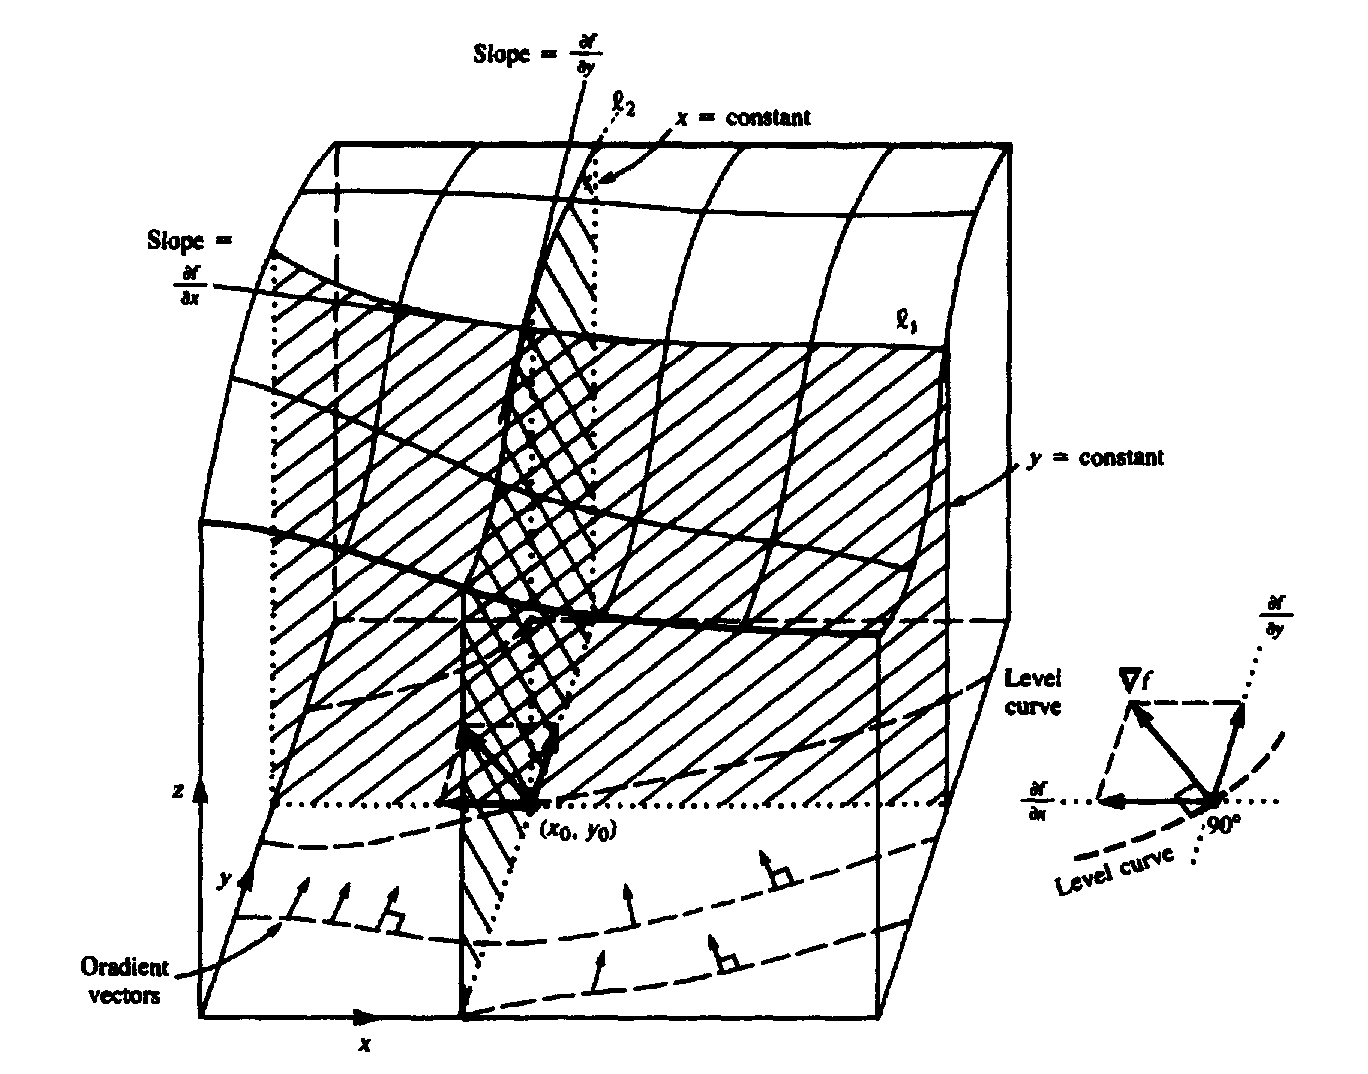
\includegraphics[scale=0.5]{figs/leah/fig09.02.png}
\label{fig:09.02}
\end{figure}


\begin{comment}
The following properties of partial derivatives follow from their basic definition: ir-cTx'
m
dx dx dx,

for functions /and g and constant c. Similar equations ensue for partial differentiation with respect to y.

For functions that are continuously differentiable sufficiently many times, it is also true that mixed partial differentiation in any order produces the same result. For example
fyx = partial \partial x(\partial f \partial y )

Note: Equation (6c) also defines the equivalent notation used for multiple partial differentiation.
\end{comment}
%\begin{comment}
As seguintes propriedades de derivadas parciais seguem de sua definição básica:
\begin{eqnarray}\label{eq:09.06ab}
\dfrac{\partial (cf+g)}{\partial x} = c\dfrac{f}{\partial x} + \dfrac{g}{\partial x},
\end{eqnarray}
para funções $f$ e $g$ e constante $c$. Equações semelhantes resultam da diferenciação parcial em relação a $y$.

Para funções que são continuamente diferenciáveis o suficiente muitas vezes, também é verdade que a diferenciação parcial mista em qualquer ordem produz o mesmo resultado. Por exemplo
\begin{eqnarray}\label{eq:09.06c}
f_{yx}
= \dfrac{\partial}{\partial x} \left(\dfrac{\partial f}{\partial y}\right)
= \dfrac{\partial^2 f}{\partial x \partial y} 
= \dfrac{\partial^2 f}{\partial y \partial x}
= \dfrac{\partial}{\partial y} \left(\dfrac{\partial f}{\partial x}\right)
= f_{xy}
\end{eqnarray}

\textbf{Nota}: A Equação (6c) também define a notação equivalente usada para diferenciação parcial múltipla.
%\end{comment}

\begin{comment}

\end{comment}
%\begin{comment}

%\end{comment}

\begin{comment}

\end{comment}
%\begin{comment}

%\end{comment}

\begin{comment}

\end{comment}
%\begin{comment}

%\end{comment}

\begin{comment}

\end{comment}
%\begin{comment}

%\end{comment}

\begin{comment}

\end{comment}
%\begin{comment}

%\end{comment}








% AQUI ESTOU PULANDO
\begin{comment}







gradients

For a function/of several variables the gradient, symbolized Vf, is a vector consisting of the partial derivatives off. For example,if/ =f(x, y), then
Uf = f(x,y,z), then
(7)
(8)
and so on for functions of n variables. The symbol V is called the del operator, and is discussed in greater detail in Section 9.3. The gradient vector has the following properties:

1. The magnitude of Vf, \\Vf |, represents the steepness of the local variations in the
function/. For example,
lYM
= (/,2+//),/2. (9)



2.

(a) The direction of V/, is a unit vector in the direction of steepest(increasing) slope, in the sense
that a step in this direction leads to the greatest increasein/per unit distance,
(b) The gradient vector at a point (xq, Vq) is perpendicular to a level curve
fix, y)
= c that goes through fa, yo) as long as (x0, yo) is not a local maximum, minimum, or saddle point.
For every point in R2 (analogously, R3 or R\") at which the function /is defined,
is continuous, and has partial derivatives, there will be a gradient vector. The vector
will have all zero components at the critical points of/.
It is common to visualize a whole collection of these vectors, one at each point in
space, as a vectorfield. A vector field that arises thus is called a gradient field and has
certain special properties. (Note that a gradient field is a vector field, but the converse
is not necessarilytrue.)

    Gradient fields can always be paired (up to an arbitrary constant) with differentiable multivariate functions and vice versa (see examples in the following boxes). We see that the variations in a spatial distribution lead to orientation cues that are represented by the geometry of the gradient field.

    The proof of the statements in this box are basedon the chain rule of functions of several variables and on the properties of curves and vector dot products. These can be found in any text dealing with the calculus of several variables.


Example1
Consider the function
fix, y) = x2 - 2x + y2 + Ay + 5.
Level curves of this function have the equation
c = x2-
-(*-
2x+ y2 + Ay + 5
D2 + (y + 2f.
These are circles of radius c'/2 centeredat the point (1, -2).
fix, y) are the following:
dx
d2f = o,
dx dy
dx2
lt
2, | = 2y + 4,
dy
*f = o,
dy dx
3y2
2'

The gradient vector at a point (x, y) is
*-(&#-*->.*
+ *
This vector is perpendicular to a level curve going through the point (x, y). A
critical point of/occurs at (1, -2), where Vf
= (0, 0). At this point,/(l, -2) = 0. At
any other point/is greater. For example,/(l, 1)= 1-2+1+4 + 5 = 9.
Therefore(1, -2) is a local minimum. (A more rigorous second-derivative test to distinguish
between local minima, maxima, and saddle points is given in most calculus books).


Example 2
Considerthe vector field
F = (M(x,
= (2x +
y), N{x, y))
2y + y cos xy,2x -\\- x cos xy).
We would like to determine whether F is a gradient field, that is
function fix, y) such mat
F
If so, then
F
whereM(x,y)
= df/dx and N =
By a previous observation
dy
fxy
Checking this, we note that
= V/.
-<\"\342\200\242\302\273-(!\342\200\242#\342\200\242
df/dy.
we must have
hx
dx'
dM \342\200\236 dN
\342\200=\224 2 + cos xy
- xy sin xy
=
 --- ,
dy
J J dx
(10)
i, whether there is a
Ola)
(Ub)
(12)
so that no contradiction results by assuming that (11a) holds. The condition given by
(12) in fact guarantees that F is a gradient field (a fact whose proof will be omitted
here).
To find /we need a function whose partial derivatives satisfy the following:
3/
dx
a/
dy
= 2x + 2y + y cos xy,
= 2x + x cos xy.
(13a)
(13b)


Integrating each expression with respect to a single variable while holding the other
variable constant leads to these results:
f(x, y)
= (2x + 2y + y cos xy)dx (14)
\342\200\242/(y-conw)
= x2 + 2xy + sin xy + H,
and
fix, y)
= (2x + x cos xy)dy (15)
J (r --- const)
= 2xy + sinxy + G.
In ordinary one-variable calculus, a single integration introduces a single arbitrary
constant. However, in the partial integration of (14) and (15) one must account for the
distinct possibility that the integration \"constants\" H and G may depend on the values
given to the fixed variables (to y = const and to x = const). For this reason it is
necessaryto presuppose that
H = h(y) and G = g(x) (16)
are functions. Indeed, the only possibility for matching the two different expressions,
(14)and (IS), both of which equal the same function/(x, y), would be to take
G(x)
= x1 + c, H(y) = c,
for constant c.
The conclusion then is that
f(x, y) = x2 + 2xy + sin xy + c. (17)
To checkthis result, observe that
Vf = (2x + 2y
- y cos xy, 2x - x cos xy)
= F,
which confirms the calculation. Note that adding any constant to f(x, y) results in the
same gradient. Thus/(x, y) is defined only up to some arbitrary additive constant.



Example 3
The concentration of nutrient particles suspended in a pond is given by the expression
c(x, y, z)
= Co exp -a(x2 + y2 + z2). (18)
An organism located at (x, y, z) = (1, -1, 1)moves in the direction of increasing
concentration. In which direction should it move? Where is the maximum concentration?
Answer
To find the direction of greatest increaseperunit distance, compute the gradient vector.
Sincec is a function of three variables, Vc is a vector in R3:
(dc dc dc\\
Vc =
\\Tx'Ty>i;)
<19a>
= (-2axC0e-'\"2,-2ayC0e-'\"1-,2azC0e-'\"1), (19b)

where
r2 = x2 + y2 + z2 (19c)
at(l, -1, 1)
r2 = 3 and Vc = (-y, y, -y),
where
y = 2aC0e-3a.
Furthermore, Vc = 0 only when (x, y, z) = (0, 0, 0), sothat the origin is a
critical point. It is readily observedthat this is a local maximum, since c(x,y, z) is a
function that decreases exponentially with distance from the origin. Thus, the maximal
concentration of nutrient particles is c(0, 0,0) = C0. We further observe that equiconcentration
loci are surfaces that satisfy
Co exp -a(x2 + y2 + z2) = constant. (20a)
After algebraic simplification this becomes
x2 + y2 + z2 = K (K = constant), (20b)
which represents spheres with centers at (0, 0, 0) and radii VAT.
Thus the organism will move in the direction of the gradient, and its path will
eventually end at (0, 0, 0).


In the next section our purpose is to understand the basic processthrough which a
partial differential description of motion through space is obtained. We shall be
concerned mainly with the dynamic processes that lead to changes in a spatial
distributioonver time. Some of the many examplescited pertain to the motion and
continuoruesdistribution of animals, cells, and molecules through space. For this reason we
shall dealwith functions that depend on both space and time

\end{comment}


\section{UMA RÁPIDA DERIVAÇÃO DA EQUAÇÃO DE CONSERVAÇÃO}


A equação de conservação em suas várias formas é a declaração mais fundamental por meio da qual as mudanças nas distribuições espaciais são descritas. A maioria dos EDP que encontraremos baseia-se basicamente nessas declarações de equilíbrio. Para obter uma familiaridade fácil com os conceitos básicos, consideraremos um caso bastante especial e daremos primeiro uma derivação informal, para posteriormente ser mais rigorosa e geral.

Nossas suposições iniciais são que:

1. O movimento ocorre em uma única dimensão espacial (como, por exemplo, no tubo fino da Figura 9.3a).

2. A seção transversal do navio ou contêiner é constante ao longo de todo o seu comprimento.

Devemos deixar $x$ representar a distância ao longo do tubo de algum local arbitrário. Fixando a atenção no intervalo entre $x$ e $x + \Delta x$, vamos descrever as mudanças na concentração, considerando dois efeitos possíveis:

(1) fluxo de partículas para dentro e fora do intervalo $(x, x + \Delta x)$ e

(2) processos que introduzem novas partículas ou degradam partículas localmente (como por meio de uma reação química).


\begin{figure}[!ht]
\caption{\small Equações de equilíbrio são derivadas para o fluxo de partículas [concentração $c(x, t)$] ao longo de um tubo, (a) Se o tubo tem área transversal $A$ uniforme, a equação (24) resulta de um equilíbrio de fluxos para dentro e para fora de uma pequena seção (b) de comprimento $\Delta x$. (c) Se o tubo tem uma área $A(x, t)$ que varia espacial ou temporalmente, obtém-se a equação (29) formulando o balanço para a pequena região mostrada em (d).}
\centering
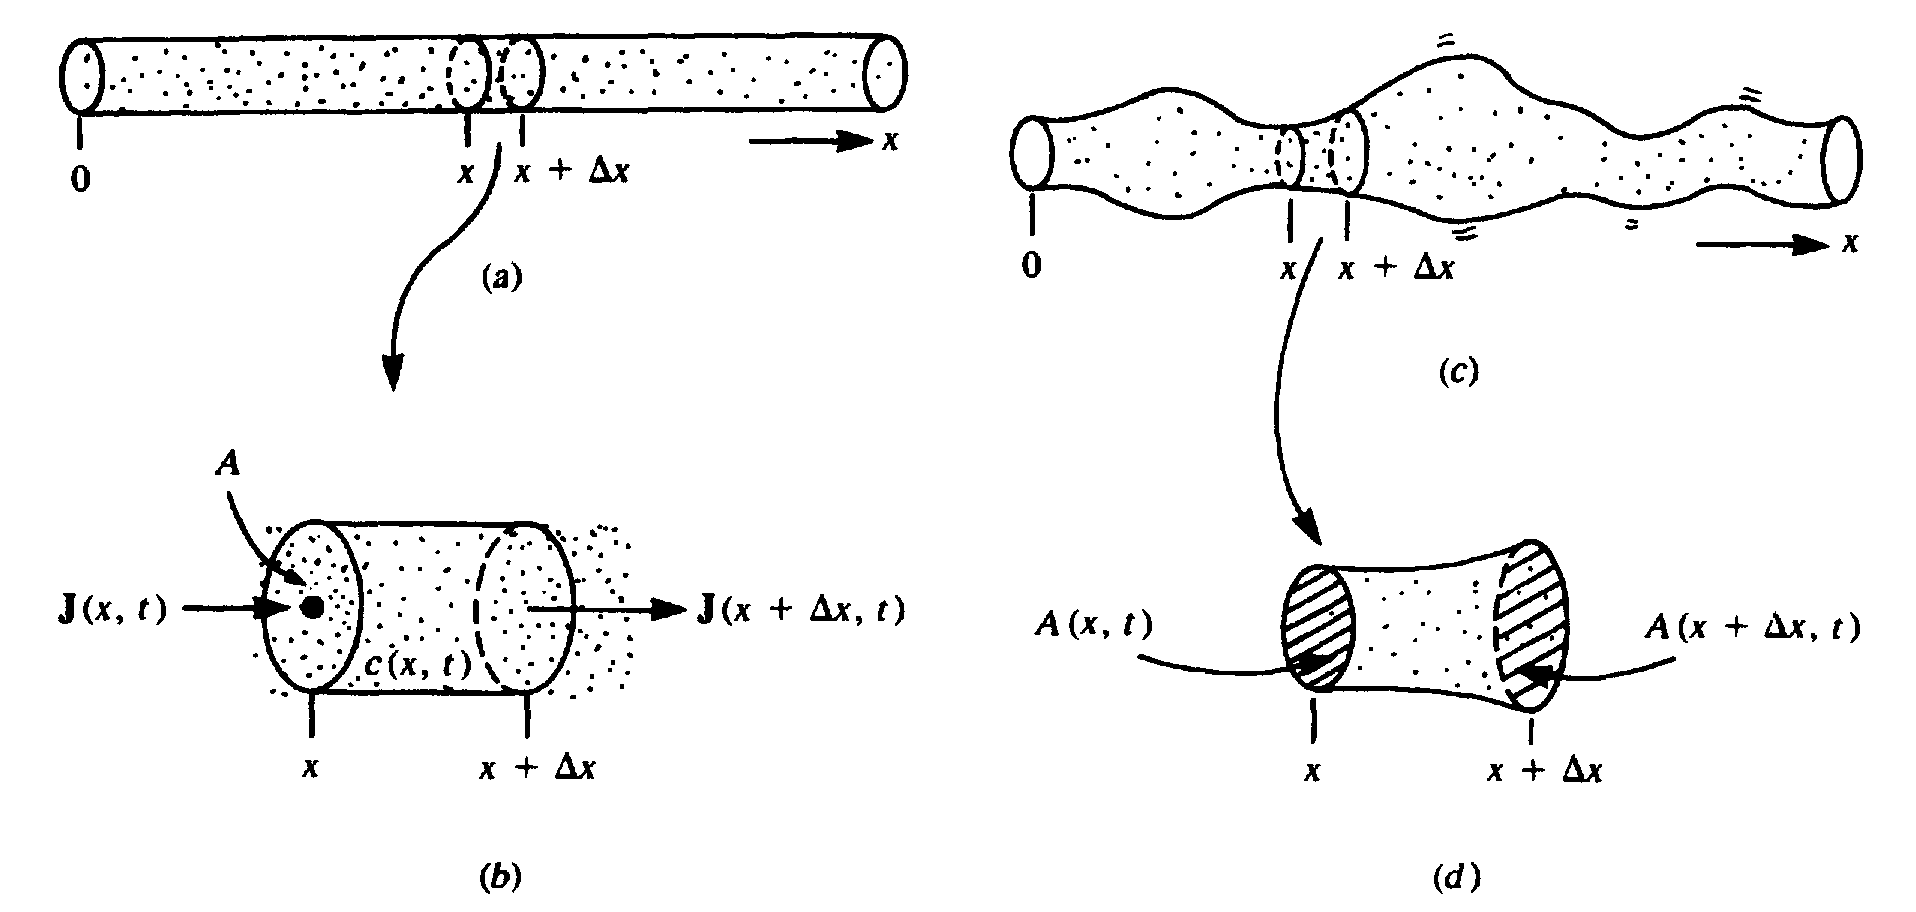
\includegraphics[scale=0.5]{figs/leah/fig09.03.png}
\label{fig:09.03}
\end{figure}

A equação de equilíbrio pode ser escrita em termos de massa ou número de partículas. Nós escolhemos arbitrariamente a última descrição e, portanto, nossa declaração será
$$
\left[
\begin{tabular}{m{0.15\textwidth}}\tiny
taxa de mudança da população de partículas em $(x, x + \Delta x)$ por unidade de tempo
\end{tabular}
\right]
=
\left[
\begin{tabular}{m{0.15\textwidth}}\tiny
taxa de entrada em $(x, x + \Delta x)$ por unidade de tempo
\end{tabular}
\right]
-
\left[
\begin{tabular}{m{0.15\textwidth}}\tiny
taxa de partida de $(x, x + \Delta x)$ por unidade de tempo
\end{tabular}
\right]
\pm
\left[
\begin{tabular}{m{0.15\textwidth}}\tiny
taxa de degradação local ou criação por unidade de tempo
\end{tabular}
\right]
$$


Para ir além, defina as seguintes quantidades:

$c(x, t) =$ concentração de partículas (número por unidade de volume) em $(x, t)$,

$J(x, t) =$ fluxo de partículas em $(x, t)$ = número de partículas cruzando uma área unitária em $x$ na direção positiva por unidade de tempo,

$\sigma (x, t) =$ densidade de sumidouro / fonte = número de partículas criadas ou eliminadas por unidade de volume em $(x, t)$.


Notamos que o único fluxo que altera a população total é aquele que entra ou sai pelas seções transversais em $x$ e $x + \Delta x$, a saber, $J(x, t)$ e $J(x + \Delta x, r)$.

Para agora traduzir (21) em uma equação dimensionalmente correta, é necessário levar em consideração as seguintes quantidades:

$A =$ área da seção transversal do tubo,

$\Delta V =$ volume do elemento de comprimento $\Delta x = A \Delta x$.

Cada termo na equação deve ter as mesmas unidades que os termos no LHS de (21): número por unidade de volume por unidade de tempo.

Isso leva à seguinte equação:
$$\dfrac{\partial}{\partial t} [c(x, t) A \Delta x]
= J(x, t) A - J(x + \Delta x, t) A \pm \sigma(x, t) A \Delta x.
%(22)
$$

Observe que, como $c$ depende de duas variáveis, sua derivada em relação ao tempo é uma derivada parcial. Escolher escrever a equação (22) em termos de $x$, a coordenada do limite esquerdo do intervalo, é totalmente arbitrário, pois estamos prestes a tomar o limite $\Delta x \to 0$.

Observamos que um fluxo na direção $x$ positiva tende a contribuir para a população líquida positivamente em $x$, mas negativamente em $x + \Delta x$; daí os sinais dos termos em (22). Veja a Figura 9.3 (b).

Agora, dividindo por $A \Delta x$, que por suposição é constante, obtemos:
$$
\dfrac{\partial}{\partial t} c(x, t) = \dfrac{J(x, t) - J(x + \Delta x, t)}{\Delta x} \pm \sigma(x, t).
%(23)
$$





Tomando o limite desta equação como $\Delta x \to 0$, como a largura da fatia fica cada vez menor, chegamos a uma afirmação local, a equação de equilíbrio unidimensional,

$$
\dfrac{\partial}{\partial t} c(x, t) = \underbrace{-\dfrac{\partial J(x, t)}{\partial x}}_{\textrm{movimento líquido}} \pm \underbrace{\sigma(x, t)}_{\textrm{fonte / dissipador}}.
%(23)
$$

O sinal negativo em $\partial J / \partial x$ deriva do fato de que a diferença finita em (23) tem um signo oposto àquele na definição de uma derivada.

Esta é a forma básica da lei de equilíbrio que em breve aplicaremos a vários problemas específicos. Antes disso, faremos uma série de extensões e declarações gerais. É possível pular este material e ir para a Seção 9.4 sem perda de continuidade.




\section{OUTRAS VERSÕES DA EQUAÇÃO DE CONSERVAÇÃO}

\subsection{Fluxo tubular}

Devemos abandonar a suposição (2) e considerar a possibilidade de que a área da seção transversal do tubo pode variar no espaço e no tempo. Para ser um pouco mais formal, tomamos as seguintes definições: Pela concentração $c(x, t)$ queremos dizer uma quantidade tal que

$\displaystyle \int_{x_1}^{x_2} c(x, t) A(x, t) dx =$ número total de partículas localizadas dentro do tubo no intervalo $(x_1, x_2)$ no tempo $t$.
%(25a)


Da mesma forma, a densidade da fonte $\sigma(x, t)$ é definida por

$\displaystyle \int_{x_1}^{x_2} \sigma(x, t) A(x, t) dx =$ taxa de criação ou degradação de partículas dentro do intervalo $(x_1, x_2)$ no tempo $t$.
(25b)
 
A equação de equilíbrio pode então ser escrita na forma integral (às vezes chamada de forma fraca), como segue:

$$
\dfrac{\partial}{\partial t} \dint_{x_0}^{x_0+\Delta x} c(x, t) A(x, t) dx 
=
J(x_0, t) A(x_0, t) - J(x_0 + \Delta x, t) A(x_0 + \Delta x, t) \pm \dint_{x_0}^{x_0+\Delta x} \sigma(x, t) A(x, t) dx.
%(26)
$$

(Isso é semelhante a uma derivação em Segel (1980, 1984) para área constante.)

Um teorema do valor médio integral permite concluir que em alguns locais
$(x_1, X_2)$ (onde $x_0 \le x_i \le x_0 + \Delta x$, para $i = 1, 2$) o seguinte é verdadeiro:

$$\dfrac{\partial}{\partial t} [c(x_1, t) A(x_1, t)] \Delta x
= J(x_0, t) A(x_0, t) - J(x_0 + \Delta x, t) A(x_0 + \Delta x, t) \pm \sigma(x_2, t) A(x_2, t) \Delta x.
%(27)
$$


Agora dividindo por $\Delta x$ e deixando $\Delta x \to 0$, obtemos $x_1 \to x_0$ e $x_2 \to x_0$, que na equação limite (27 ) torna-se


$$\dfrac{\partial}{\partial t} [c(x_0, t) A(x_0, t)]
= -\dfrac{\partial}{\partial x} [J(x_0, t) A(x_0, t)] \pm [\sigma(x_0, t) A(x_0, t)].
%(28)
$$

\subsection{Casos especiais}



1. Se $A(x_0, t) = A$ for constante, dividir por $A$ reduz a equação (28) à equação (24).

2. Se $A(x, t) = A(x) \neq 0$ (ou seja, se a área não muda com o tempo), a equação pode ser escrita na forma
$$
\dfrac{\partial}{\partial t} c(x, t)
= - \dfrac{1}{A(x)} \dfrac{\partial}{\partial x} [J(x, t) A(x)] \pm \sigma(x, t).
%(29)
$$

Quando a derivada parcial é expandida, obtém-se:
$$
\dfrac{\partial}{\partial t} c(x, t)
= - \dfrac{\partial}{\partial x} J(x, t) - \dfrac{J(x, t)}{A(x)} \dfrac{\partial}{\partial x} A(x) \pm \sigma(x, t).
%(30)
$$


A equação é, portanto, semelhante a (24), mas contém um termo extra que explica um efeito semelhante à diluição; ou seja, uma mudança na concentração que decorre de mudanças locais no volume do fluido "sentido" pelas partículas à medida que se movem ao longo do comprimento do tubo.

3. Se $A(x, t) = A (t) \neq 0$ (se a área do tubo for uniforme ao longo de seu comprimento, mas possivelmente variando no tempo), então a equação (28) leva ao seguinte:
$$
A(t) \dfrac{\partial}{\partial t} c(x,t) + c(x,t) \dfrac{\partial}{\partial t} A(t) = - A(t) \dfrac{\partial}{\partial x} J(x,t) \pm \sigma(x,t) A(t).
%(31)
$$

Depois de alguns rearranjos, isso se torna:
$$
\dfrac{\partial}{\partial t} c(x,t) = - \dfrac{c(x,t)}{A(t)} \dfrac{\partial}{\partial t} A(t) - \dfrac{\partial}{\partial x} J(x,t) \pm \sigma(x, t).
%(32)
$$

Mais uma vez, a equação se assemelha a (24), com um termo adicional que, grosso modo, também descreve um efeito de diluição conforme o tubo se expande ou se contrai.

4. Em uma situação onde a área da seção transversal varia tanto espacialmente quanto temporalmente $[A = A(x, t)]$, segue-se que a equação (28) pode ser escrita

dc (x, t) _ dj (x, t), 1 L, .i dA (x, t)








\begin{comment}








Flows in Two and Three Dimensions

To write a balance equation analogous to (24) in higher dimensions we consider a
small rectangular element of volume AV =
AxAyAz situated in R3 and account for
motion of particlesinto and out of the region. First it proves necessary to extend
somewhatour definition of flux, for now both direction and magnitude of flow have
to be considered.
Let us focus attention on a point (xo, yo, z0) in R3. We shall define flux by
counting the number of particlesperunit time that traverse an imaginary unit area A
suspended at (xo, yo, z0) with some particular orientation. As the orientation of the
\"test area\" is varied, the rate of crossingschangesIn.deed, the highest rate of
crossingis achieved when the predominant flow direction is orthogonal to the area that it
must cross. This leads us to defineflux as a vector in the direction n whose
magnitudeis given by:
net number of particles crossing
I J(*, y> z, t) I = a unit area at (x, y, z) per (34)
unit time at time t
where n is the unit normal vector to that element of area that admits the greatest net
crossings. [See Figure 9.4(a).]
We shall symbolize the components of J (in R3) as follows:
J(x, y,z) = (Jx,Jy, Jt). (35)
Each of the components Jx, Jy, and Jz may in general depend on both space and
time.
In three dimensionsthe magnitude of flux is given by the quantity
I j |
= {Ji + p, + W2 = (j \342\200\242
j),/2 (36)
(where
-
represents a vector dot product).Given some test area A, this definition of
flux allows one to calculate the number of particle crossings N that take place in a
given time f. If m is a unit vector perpendicular to the test area, one obtains
N= (J-m)A Ar. (37)



Figure 9.4 \caption{(a)In R3 flux J is a vector. Its
magnitude represents the net number of particles
crossing an imaginary unit area per unit time. Its
direction is given by the normal vector n to the
given area A. (b) Theequation of conservation
(39) is derived by considering net flow into a small
rectangular volume of dimensions Ax X Ay X Az.}



To illustrate this idea, considera wall of unit area at the point (-1,0, 3) orthogonal
to the direction m = (1, 0, 0),and a flux J = (z -
y, x  --- 
z, y
 --- 
x). At the point in
question,
J = (3, -4, 1),



so that the number of crossings is
N = (J m) lAr = [(3, -4, 1) \342\200\242
(1, 0, 0)] At = 3At.
Thus three particles traverse the wall per unit time.
Given a small rectangular volume as shown in Figure 9.4(b), the statement of
balancemust accommodate, as before, local creation and entry or departure through
each of the six planar surfaces. Since these planes are parallel to the coordinate
planes, we can readily determine their normal vectors and calculate the net number
of particles crossing (inwards) through each wall. (See Table 9.1.)
The net rate of change of concentration inside the volume that accrues from
combining all thesefactors is the following:
dc _ Jx(xq, y0> zo)
- Jx(xp + Ax, yo, z0)
dt Ax
. /y(*o> yo. zo) -
4\302\273(*o>yo + Ay. z0)
Ay
+
Uxo,yo,zo)-Uxo,y0,z0 + Az)
\302\2^61 ^ ^ ^
Taking the limit as Ax \342\2000,\224*A\3y42\226\240 -*\342\022,6\24a0nd Az \342\2000,\224o*ne obtains
dc
dt
(dJx dJy dJ,\\
-
=
-\\Tx+-o-y-
+
Tz)\302\261a{x>y>z)-
<39)
|=-V-J\302\261cr (40)
where V \342\200\242 J, called the divergence of J, is the parenthetical term in equation (39).
This scalarquantity can be described roughly as the net tendency of particlesto
leave an infinitesimal volume at the point (x, y,z). Moredetails about the del
operatorV are given in the box.
We have completedthe derivation of the three-dimensional conservation
equation. Note the similarity of equations (40) and (24). The two-dimensional case is left
as an easy exercise for the reader. We must next turn to the question of what induces
the motion of particles, molecules, or organisms so we can relate the idea of flux to
the functions mat describe spatial distributions.



Table 9.1 Particles Entering the Box (SeeFigure 9.4b.)
Wall
number
1
2
3
4
5
6
Location
on the plane
x = xo
x = Xo + Ax
y =
yo
y
= yo + Ay
z = Zo
z = zo + Az
Inwards
normal vector n
(1, 0, 0)
(-1,0,0)
(0, 1,0)
(0.-1.0)
(0, 0, 1)
(0,0,-1)
Net inwards
crossing J \34n2\226\240
Jx(xo, yo, zo)
-JxUo + Ax, yo, zo)
\342\200\24y2oM,*o>zo)
-Jy(x0, yo + Ay, zo)
\342\200\24y2oJ*, (*oz.o)
~Jz(xo, yo, zo + Az)



The Del Operator V
Loosely speaking, the quantity V behaves like a vector whose components in R3 are
\302\273 (d d V = d\\
{TX'Vy'Yj-
(41>
We can think of the componentsas partial derivatives \"hungry for a function to
differentiate.\" The del operator can be combined with vector or scalar functions in several
ways that parallel standard vector operations, as shown in Table 9.2.


Table 9.2 Analogies between Vector and Del Operations
Ordinary vector operations Analogous del operations
Scalar multiplication
Dot products
Cross products
For v = (t?i, u2, v-i) and a scalar a,
av = (at?i,at?2, av-*).
The result is a vector.
For v = (t?i, v2, u3) and
u = (m,, m2, m3),
V-U = V\\U\\ + V2U2 + U3M3.
The result is a scalar.
For two vectors v and u as defined
above,
(i
J k
V X O = I Vi V2 U3
\\Ml \302\2532U3/
=
(U2\302\2533
-
M2U3, \302\2533\302\2531
_
U|\302\2533,
\302\253l\302\2532
 --- 
t?2\302\253l).
The result is a vector.
For V as defined in (41) and a
functionf{x, y, z),
w=(\302\261
' i- i-V \\a*'dy' dz//
= fif if K)
\\dx' dy' dz/'
This is the gradient of/ and is a
vector.
For V as defined in (41) and
V = (t?|, U2, t?3),
V-v = (A A i^
\\&c' dy' dz)'
(vt, V2, V))
_ dvi dv2 , df3
d* dy dz
'
This is the divergence of the vector
field v and is a scalar quantity.
For V and v as defined above,
V x v =
dt)2 dv\\ _ \302\247V3
dz
' dz dx'
dv2
dx dy)'
This is the curl of the vector field v
and is a vector.


In descriptive terms, the vector Vf measures local variations in a function and
points to the direction of greatest steepness. The scalarquantity V - v measures the
tendency of a vector field to represent the divergence (departure) of a fluid; the vector
V x v (called the curl of v) depicts a magnitude and axis of rotation (for example, of
fluid in a vortex). Figure 9.5 demonstrates several vector fields that have net curl or
divergence. We shall not concern ourselvestoo greatly with curl since in biological
situations rotation is rarely encountered. (It does play a role in other physical sciences such
as meteorology, where rotating atmospheric flows can be viewed as generating
turbulentstorms.) As equation (40) indicates, however, divergenceis more relevant since
we attempt to keep track of changes in densities of biologicalsubstances or
populations.More details and basics about the properties of vector fields and the operations on
them can be obtained in most standard calculus texts.


Figure 9.5 Several examplesof vector fields
depicting such properties as divergenceand ///
rotation of particles, (a) V \34v2\20#0\2420 and * / , /
V x v = 0. (b)V- v = QandV x v \302\206.1 / '
(c)V
\34v2\22*6\2400 and V x v # 0. (d) V
\34v2\22*6\2400 *
and V x v = 0 (atpoint V). (e) V \34v2\20=0\2402
and V x v = 0.



Example 4. Propagation of the Action Potential Along an Axon
In Section 8.1 equation (9) was derived for the action potential in the membrane of a
voltage-clampednerve axon. (Recall that voltage clamping means keeping the voltage
the same all along the axon.) In real axons the action potential is a signal that
propagates from the soma (cell body) along the axon to the terminal synapses. A spacedependent
model must take this into account. Here we derive a balanceequation for
charge that incorporates the effect of transport in the axial direction. Define
x = distancealong axon,
q(x, t) = charge density per unit length inside axon at location x and time t,
J(x, t)
= flux of charged particles (= current) at location x and time t.
cr(x, t)
= rate at which charge enters or leavesaxon through its
membrane at (x, t).
By referring to Figure 9.3 and to equation (24) one concludesthat q is governed by the
equation
da BJ
i
=
~Tx + (T- <42>
(See problem 18.) In Section 8.1 we established that
qix, t) = 2iraCv(x, t), (43)
where
C = the capacitance of the axonal membrane,
a = the radius of the axon,
v = the voltage across the membrane.
It has further been shown that the rate at which charge enters the axon is
cr(x, t) = -lirah, (44)
where /, is the net ionic current into the axon. Note that a is analogous to a local source
of charge. (It is the only term that leads to changes in q in the voltage-clamped
equation (6) of Section 8.1.)
To find an expression for J we now use Ohm's law, which states that the current
(in the axial direction) is proportional to a voltage gradient and inversely proportional
to the resistanceof the intracellular fluid. This implies that the net axial current in the
axon would be
\342\2\30402\2\22040\224('7ra2\\
^v
\\R~)~dx
(45)
where dv/dx is a local voltage gradient and R is the intracellular resistivity (ohm-cm).
Making the appropriate substitutions leads to the following equation for voltage:
dt 2RC dx2 C\"
' '
(Seeproblem 18.) This equation with the appropriate assumptions about /, is used to
study propagated action potentials.


CONVECTION, DIFFUSION,AND ATTRACTION
Equations (24) and (40) are general statements that apply to numerous possible
situations. To be more specific, it is necessary to select terms for J and <r capturing the
particular forces and effects that lead to the motion, and to the creation or
elimination of particles. The choices may be madeon the basis of known underlying
mechanisms, suitable approximations, or analogy with classical cases. We deal here with
three classical forms of the flux term J.
Convection
Particles in a moving fluid take on the fluid's velocity and participate in a net
collectivemotion. If v(x, y, z, t) is the velocity of the fluid, one can easily demonstrate
that the flux of particles is given by
J = cv, (47)
where all quantities may vary with space and time. (See problem 10for the key idea
in proving this.)
Substituting (47) into equation- (24) leads to the following one-dimensional
transport equation:
dc(x,t) d r - . . , ., . .\342\200\236.
dt
= ~
Tx[c(*'r)v(*' ^' ( *
or, in arbitrary space dimensions,
ft
= -v-(cy). (49)
Attraction or Repulsion
Suppose iff is a function that represents some sourceof attraction for particles. (For
example, the particles could be charged,and 4> could be an electrostatic field.) An
attractive force would pull particles towardsthe site of greatest attraction. The
direction and the magnitude of motion would thus be determined by the gradient of \\j/ (for
example, it might be aVtp for somescalara); the net flux in that direction would be
J - caVtl/. (50)
(In one dimension this is simply J = ca(d\\]//dx).) Substituting into equation (24)
results in the following one-dimensional equation for attraction to ifi:
dc(x, t) d [ , dtff]
....


Random Motion and the Diffusion Equation

One of the most important sources of collective motion on the molecular level is
diffusion, which results from the perpetual random motion of individual molecules.
Diffusion is an important \"metabolically cheap\" transport mechanism in biological
systems, but as we shall see, its effectiveness decreases rapidly with distance. A
familiar assumption made in the context of diffusion through cell membranes is that
the rate of flow depends linearly on concentration differences. This is an
approximattoion a more complicated situation. An extension of this concept to more general
situations is known as Fick's law, which states that the flux due to random motion is
approximately proportional to the local gradient in the particle concentration:
J = -3Vc. (53)
Theconstant of proportionality 2) is the diffusion coefficient. The net migration
due to diffusion is \"down the concentration gradient,\" in a direction away from the
most concentrated locations. This makes sensesincein most situations where there
is a relatively large local concentration, more molecules leave on average than return
(due to the random character of their motions).
In one dimension, diffusive flux is simply given by J = -2)(dc/dx), so that
upon substitution into equation (24) one gets
dc(x,t) d_
dt dx ix^'t]
9 -
c(x, t) (54)
(If 2> is a constant and does not depend on c or x, it can be drawn outside the outer
derivative, giving the most familiar version of the one-dimensionaldiffusion
equation:
dc _ d2c
\342\20=0\2242)  --- 
dt dx 1--9T3. (55a)
In arbitrary dimensions this result would be written
or, if 2> is constant, then
jt
= V \342\226\240
(2>Vc), (55b)
^ = 2) Ac = 2)V2c. (55c) dt ' '


Random Walk and the Diffusion Equation
A collection of particles shown in Figure 9.6 moves randomly with an average step
length Ax every time unit r. Assume that the probability of moving to the left, A,, and
to the right, Ar, are both equal; that is, A, = Ar =
\\. The x axis is subdivided into
segments of length Ax. We write a discrete equation that describes the change in the
numberof particles located at x.
J_
x \342\A20x0\224 x x + Ax
Figure 9.6 Particlesarrive at or depart from moving left or right.
x randomly, with probabilities k> and Ar of
Let C(x, t) Ax be the number of particles within the segment [x, x + Ax] at time
t. Then
C(x, t + t) = C(x, t) + ArC(x
- Ax, t) - ArC(x, t)
+ A,C(x + Ax, t)
- A,C(x, t). (56)
Now we write Taylor-series expansions of these terms, as follows:
d\302\243 1_PC
dt
T
2 dt2 C(x, t + t) = C(x, t) + \342\200r\22+4 -
 --- j t2 +
C(x \302\2A6x1, t) = C(x, t)\302\261^-Ax
+~2C
(57)
Substituting into (56) and using the fact that A, = A; =
\\, we obtain
3c 1 d2c , 1 d2c . , 1 d*c A ,
_t + __t2+...=__^+__A^+.... (58)
Dividing through by t, we look at a limiting form of this equation for t -\302\207,3 Ax -* 0
such that
(Ax)2
It
Then the result is
= constant = 2). (59)
dt 2t dx2 dx2
' '
Note that (60) is equivalent to equation (55a).
Extensions of the random walk model for A( ^ Ar and for numerous other special
cases are described by Okubo (1980).


The symbol A is the Laplacian of c; it stands for the combination V \34V2\200(\2r4e2ad \"div
dot grad\,") also written V2. Equations (54) and (55a) are alsoknown as heat equa


tions since they describe equally well the diffusion of heat following Newton's law
of cooling.
Fick's law is just one version of flux of diffusion and warrants several remarks.
Clearly the term \3422\2>0V0\c224 gives a directionality to J. The diffusion coefficient 2)
represents the degree of random motion (how \"motile\" the particles are); 2) depends
strongly on the size of the particles, the type of solvent, and the temperature.
While the assumption is common that diffusive flux takes the form of equation
(S3), this is not the only possibility. From a consideration of the Taylor series,
diffusive flux can be appreciated as a reasonablefirst approximation. Since diffusion
derives from concentrationdifferences,considerthe Taylor-series expansion
c(x + A*, t)
 --- 
c(x, t)
. dc (tfx\\ d2c
If flux depends linearly on differences in concentrations, for quite small Ax, it is
approximately proportional to dc/dx, which is the one-dimensionalversion of (53).
In more complicated situations (chiefly for high concentrations when
interactions between molecules become important), Fick's law is no longer accurate and
other versions of diffusion are more applicable.It is a challenging physical problem
to deal with such situations. A full treatment of the diffusion equationand of random
walks is given in Okubo (1980) along with references and outlinesof its extensionto
more complicated situations.
9.5 THE DIFFUSION EQUATIONAND SOME OF ITS CONSEQUENCES
The one-dimensionaldiffusion equation derived in Section 9.4 is
dt dx
T1
=
\302\256TT2- P5a)
In radially and spherically symmetric cases in two and three dimensions the
equation is slightly different: In two dimensions one obtains
3c _ 2) d ( dc\\
Tt-77ArTr)' (61>
whereasin three dimensions the result is
dt-R*dR\\R Skh (62)
where r and R are the distances away from the origin. (See problem 12 for an easy derivation.)

The methods one would apply to solving each of these equations would be
somewhat different. However, even without solving them explicitly, certain
interestincgonclusions can be made. Based on dimensional considerations alone it follows
from any one of equations (55a), (61), or (62)that 2> has the following units:
_ (distance^
time
'

Table93 Diffusion Coefficients of Biological Molecules
Temperature(\302\260C)
0
20
18
25
20
Substance
Oxygen in air
Oxygen in air
Oxygen in water
Oxygen in water
Sucrose in water
%(cm2 sec~')
1.78 x 10\"'
2.01x 10-'
1.98x lO-5
2.41 x 10\"5
4.58 x 10\"6
Ref
1
1
1
1
2
Sources:
1. L.Leyton (1975), Fluid Behavior in Biological Systems, Clarendon Press, New York.
2. K. E. Van Holde (1971),Physical Biochemistry, Prentice-Hall, Englewood Cliffs, N. J.


From this simple observation follow a number of results whose consequencesare
important in numerous biological systems. First, as we shortly see, equation (63)
implies that
1. The average distance through which diffusion works in a given time is
proportional to (2>f)1/2-
2. The average time taken to diffuse a distance d is proportional to d2/(3>.
The diffusion coefficients of several key biological substances are given in
Table 9.3. As a typical magnitude for the diffusion coefficient of small molecules
such as oxygen in a medium such as water, we shall take
2>oxygen
=* 10\"5 CHI2 SeC-1 .
The dimensionsof a singlecellareroughly 1 to 10 microns (1 fi = 10\"4 cm =
10~6 m). As shown in Table 9.4, the amount of time it takes to diffuse through a
given distance increasesrapidly with the length scale.
On the scale of intracellular structures, diffusion is an extremely rapid process
and can thus act as a metabolicallyfree transport mechanism, in the sense that no
energy need be expended by the cell to maintain it. On somewhat larger scales, (such
as 1mm),diffusion is already inadequate for such criticalfunctions as oxygen
transport. The longest cells of the human body are neurons; some of these have axons
that are at least 1 m in length. Transport of small molecules from one end to the
other would take roughly 30 years if diffusion were the only available mechanism.
Table 9.4 Time Taken to Diffuse Through a Given Distance
Distance Diffusion time
1 um = 10-6 m 10\"3 sec
10 um 0.1 sec
1 mm 103 sec = 15 min
1 cm 103 sec = 25h = 1 day
1 m 108 sec \342\22070\22y4ears


The following simple arguments due to, for example, Haldane (1928) and LaBarbera
and Vogel (1982)lead to a number of deductions about the limitations of
diffusion.
Consider a spherical cell of radius r. The volume and surface area of such a
cell are
V =
|7rr3, S = 4tjt2. (64)
Supposethat the cell metabolizes a given substancecompletely, so that its
concentration at r = 0 is c(r, t)
= 0, while its concentration at the surfaceis c0.The
gradientthus established is co/r (concentration differenceperunit distance). Thus a
diffusive flux of magnitude 2>co/r would admit moleculesthrough the cell surface. The
total number of moleculesentering the cell per unit time would be
JS = 2)- 47JT2 =
47r2>c\342\200\236r. (65)
The rate of degradation of substance,however, is generally proportional to the
volume of the cell:
4 7JT3 y,,% rate used = , (66)
where t is the time constant for the degradation process. Thus
^^^32>co^. (67)
rate used rz
Since for a viable cell this ratio should not fall below 1, it is necessary that
1-32)co 4r'. (68)
or
To match supply and demand the minimum external substance concentration must be
proportional to the square of the cell radius. It is therefore unrealistic to expect
spherical cells whose radii are largeto rely solely on diffusion as a means of
conveyincgrucial substances inside the cell.
LaBarbera and Vogel (1982) point out some of the most common ways
adopted by organisms to reduce the limitations due to diffusion. These are
highlighted below.
shape
Geometry influences diffusion rates. Flat shapes (such as algal leaves) or long
branched filaments (such as fungi, filamentous algae, roots, and capillaries) are
ideally suited for organisms that rely heavily on direct absorption of substances from
their environment; these shapescan increasein volume (for example, by getting
longer) without changing the distance through which diffusion must act (that is, the




radius of the cylinder). La Barbera and Vogel suggest a dimensionlessflatness
index
S3
7 = (70)
as an appropriate description of shape; they point out that with increasing size, an
organism relying on diffusion must increase its flatness.
Dimensionality
It can be shown that the diffusion time taken to reach someinternal sink depends
differently on length scales in one, two, and three dimensions; one obtains somewhat
different results from the equations (55a), (61),or (62).With the geometries given
in Figure 9.7 one can establishthe results that the diffusion time is as follows:
in one dimension: ti =
in two dimensions: T2
in three dimensions: T3=
22),'
D , L
Mlna-
L2 2L
22)33a'
(71a)
(71b)
(71c)




Figure 9.7 The average time it takes a particleto
diffuse from a source to a sink, called the transit
time t, depends on the dimensionality, (a) In one
dimension, t is proportional to V where L is the
distance, (b) In two dimensions, t is greater by a
factor of In (L/a) where a is the radius of the sink,
(c) In three dimensions the multiplicative factor is L/a. [From Hardt, S. (1980). Transit times.
Fig. 6.2.1,p.455.Copyright \302\2159180 by
Cambridge University Press and reprinted with
their permission.] In L. A. Segel, Mathematical
Models in Molecular and Cellular Biology.
CambridgeUniversity Press, England.

Here L is the cell radius and a is the radius of an internal sink (for example, an
enzyme molecule that degrades substance). (See details in Figure 9.7 and Section 9.6.)
Murray (1977, chap. 3) gives an in-depth analysis and application of the
effects of dimensionality to the antenna receptors of moths. In a set of papers,
S. Hardt describes a convenient way of calculating transit times without explicitly
solving the time-dependent diffusion equation.
We thus see that diffusion acts much more quickly in one- or two-dimensional
settings than in three dimensions. This provides an advantagefor intracellular
organization of chemical reactions on membranes (which are two-dimensional) rather
than on \"loose\"enzymes in the cytoplasm. Hardt (1978) compares the two- and
three-dimensional cases where a represents the dimensionsof an enzyme ( --- A1)0
and 2>2  ---  1002b. She concluded that for the cells of diameter larger than 1 fi, the
organism benefits by arranging enzymes on internal membranes.
Circulatory systems
Where geometric solutions to diffusion limitations have failed, organisms have
evolved ingenious mechanisms to convey substances to their desired destinations.
From the intracellular cytoplasmicstreaming and assorted mechanochemical
methods to the circulatory system of macroscopicorganisms, the ultimate purpose is to
overcome the deficiency of long-distance diffusion and to transport substances
efficiently. A fascinating account of the minimal design principlenecessaryto make
a circulatory system work is given by LaBarbera and Vogel.

9.6 TRANSIT TIMESFORDIFFUSION

Despite limitations on large distance scales, diffusion is of great importance in many
processes on the cellular level. To give one example, communication between
neighboring neurons is based on a chemical information system. Substancessuch as
acetylcholine (called a neurotransmitter) are released by vesicles at the terminal
branches of a given neuron, diffuse across the synapses, and relay messages to the
neighboring neuron. An important consideration, particularly so in this example, is
the average length of time taken to diffuse a given distance and how this time
depends on particular features of the geometry.
Until a recent innovation suggested by Hardt, the problem of diffusion transit
times was addressed by solving the time-dependentdiffusion equation in the
geometroyf interest and using the resulting solution to derive a relationship.This process
tends to be rather cumbersome for all but the simplest cases because solving
diffusion equations in complicated geometries is a nontrivial task. Thus the approach was
less than ideal.
A simpler method, proposed by Hardt (1978), is based on the observation that
the mean transit time t of a particle is independent of the presence or absence of
other particles (given that no interactions occur) and can thus be computed in a
steady-state situation. Hardt remarked that t is then given by a simpleratio of two
quantities that can be calculated in a straightforward way once the steady-state
diffusion equation is solved. Solving the latter is always easierthan solving the time-dependent problem, sinceit is an ordinary differential equation. To establish Hardt's result we define the following quantities:
N = total number of particles in the region,
F = total number entering the region per unit time,
A = average removal rate of particles,
t = 1/A
= average time of residency in the region.
Regardless of spatial variations, one can make an approximate general
statement about the total number of particles in a given region. For instance, if particles
enter at some constant rate F and are removedat a sink with rate A, then
dN _ entering _ removal _ \342\_200\23.6
N
._-.
dt rate rate
In steady state (dN/dt = 0) we obtain the result that
F = \\N = - =>r =
\302\243. (73)


Example 5
Consider the one-dimensional geometry shown in Figure 9.7(a), with particles entering
at x = L and diffusing to x = 0. Then assuming particles cannot leave the region (the
interval [0, L]), the mean residency time for a particle is the same as the mean time it
takes to diffuse from the source (wall at x = L) to the sink (at x = 0). (It is assumed
that particles are removed only at the sink.)
The time-dependent particle concentration is given by equation (55a). However,
according to Hardt's observation, to compute the mean time for diffusion it suffices to
find the steady-state quantities. To do so we consider the steady-state equation
|^-;j(-\304,2\200\242\302\243)-*
04)
and assume that c(L) = Co,c(0) = 0. (These are boundary conditions, to be discussed
in more detail in Section 9.8 and the Appendix. In the equation to be solved c depends
only on x, so we have an ODE whose solution is easily found to be
c(x) = ax + p. (75)
By using the boundary conditions we find a = Co/L and )8
= 0, so that
cW
=
Co|.
(76)
(See problem 21.) The total number of particles is
Particlesenter through x = L due to diffusive flux,
dx
Assuming a wall of unit area at x = L, we obtain the result that
F = fluxxarea=/xl= 9-2. (78)
i-i
Note that in higher dimensions it will be necessary to take into account the area
through which particles can enter, which dependsin a less trivial way on the geometry
of the region (see problems 19 and 20).
Thus the mean transit time from source to sink is
7 = N=CoL _L_ = \302\243_
F 2 9C\342\200\23629\"
' '

Derivations of similar results for two and three dimensionsare outlined in the
problems.

9.7 CAN MACROPHAGES FIND BACTERIA BY RANDOMMOTIONALONE?
Macrophages are cells that are implicatedin a number of defense responses to
infection in the body. One of their important roles is to clear the lung surface of the
bacteria we inhale with every breath. Macrophagesare motile, crawling about on the
walls of alveoli (the small air sacsin the lung at which gas exchangewith the blood
takes place) until they locate and eliminate an invader. Although the whole process
is a complicatedoneinvolving several types of cells and chemical intermediates,the
basic goal can be summarized simply:the macrophage response must be sufficiently
rapid and accurate to prevent the proliferationof invading microorganisms. A good
summary of the macrophageresponseto the bacterial challenge is given by Lauffenburger
(1986)and Fisher and Lauffenburger (1986).
These authors propose an interesting question regarding the motion of the
defending macrophages: Is random motion by the macrophages adequate to find their
bacterial targets before rapid population increase has occurred? To answer this
question, Lauffenburger observes that a macrophage moves at a characteristic speed s.
The direction of motion is typically fairly constant for a time duration r, and then
some reorientation may occur. If the motion is truly random, it is possible to define
an \"effectivediffusion coefficient\" for macrophages.
2) = $ts2. (80)
(This can be based on rigorous random-walkcalculations; see problem 22.)
We now consider a simpletwo-dimensional geometry such as the one shown in
Figure 9.1(b). The sink (or \"target\") will represent a bacterium, assumed to have an
approximate radius of detection a, and the disk (with radius R) will depict the
surface of an alveolus. We shall assume that a macrophage enters the region through its
circular boundary and searches until it arrives at its target. The transit time based on
a purely random motion is given by equation (71b). According to Lauffenburgerand
Fisher (1986), the values of constants that enter into consideration are as follows:
a = radius of bacterial cell = 20 /x,


s = speedofmotion of macrophage
= 3 fi min-1
e = time spent moving in given direction = 5 min,
A = area of alveolus = 2.5 x 10s/x.2,
N = number of bacteria = 1,
v =
reproductive rate of bacteria = 0.2 hr_l.
Then the radius of the disk is
HeM^vT-\"* \302\253>*
The effective diffusion coefficient is
3=^=(3jLi)2x^-m^
= 22.5jLi2min-1. (82)
Thus the average time to reach the bacterial cell is
L2 , L (2.8 x 102)2,2.8X 102 .\342\200\236.
T\"\302\273taA\" (2)(22.5) ln~l0 --- '
(83)
= 1.74 x 103 (2.64)
\302\247.36 x 103 min = 76 h.
However, the bacterial doubling time t* is given by
Thus if random motion was the only means of locomotion, the macrophage would
on average be unable to find its target before proliferationof bacteria takes place.
By contrast, if macrophagesare perfectly sensitive to the relative location of
their targets, the time taken to reach the bacteria would be
T = -s = 2.8 x ^3- = 93 min - 1.5 h. (85)
In practice, neither one of these two extremes is totally accurate; the
orientationof the macrophage is indeed governedby gradients in chemical factors produced
as byproducts of infection, although some random motion is also present.We shall
discuss chemotaxis more fully in the following chapters.
9.8 OTHER OBSERVATIONSABOUT THE DIFFUSION EQUATION
In this section we make some general observationsabout the mathematical properties
of the diffusion equation, leaving certain technical details to the Appendix at the end
of this chapter.
Considerthe one-dimensional diffusion equation
dt dx ^ = 2> ~2 c. (86)


By a solution to equation (86) we mean a real-valued function of (x, t) whose partial
derivatives satisfy (86). We first remark that (86) is linear. Thus if c =
<f>t(x, t) and
c =
<f>2(x, t) are two solutions of (86), then so is c =
A<f>t(x, t) + B<t>2(x, t). This
follows from the superposition principle, as in linear difference or differential
equations.
We can reinforce the connection between partial and ordinary differential
equations by writing (86) in \"operator notation\":
Jt
= 2c, (87a)
where
2 =
\302\256\302\243i-
(87b)
X is a linear operator, alsocalledthe diffusion operator; it is an entity that takes a
function c and produces another function (2) x the second x partial derivative of c).
It will soon be clearwhy such notation is helpful.
Equation (86) has two spatial derivatives and one time derivative.Thus, in
order to select out a single (unique) solution from an infinite class of possibilities, it is
necessary to specify,in addition to (86), two other spatialconstraints (boundary
conditions) and one time constraint (an initial condition). However, were this done in an
arbitrary or haphazard way, the problem might be such that no sensible solutionsto
it would exist. (\"Sensible\" solutions are those that conform to real physical
processes.) The problem is then said to be ill posed.What constitutes a well-posed
problem depends on the character of the PDE and the combination of added
conditions. (Mathematicians are particularly concerned with proving well-posedness,
since this is essentially equivalent to guaranteeing that a unique and meaningful
solution exists.) We shall avoid this issue entirely since it is beyond our scope.
Several examples of initial and boundary conditions typically applied to
equation (86) are given in the Appendix. Physically such conditions specify the initial
configuration [the concentration at time zero at every point in the region, c(x, 0)]
and what happens at the boundary of the domain. It makes intuitive sense that both
factors will influence the evolution of the concentration c(x, t) with time. For
example, a region for which particles are admitted through the boundaries will support
different behavior than one that has impermeable boundaries.
In forming solutions to the diffusion equation, one finds especially useful
functions f(x) that satisfy the relation
3T-V, (88)
where 3? is given by (87b). Such functions are called eigenfunctions, and here again,
in terminology previously encountered, A is an eigenvalue. Eigenfunctionsof the
diffusion operator have the property that their second derivative is a multiple of the
original function. Three familiar functions that fall into this category are the
following:
/,(*)
= exp (\302\261VLc), (89a)
f2(x) = sin (\302\261VXx), (89b)
f3(x)
= cos (+VA*). (89c)


By straightforward partial differentiation, the reader may verify that
c{x, t) = eKtMx) (i = 1, 2, 3) (90)
are solutions to (86) if the constantK is chosenappropriately [see problem 15(a,b)].
We arrive at the same result in the Appendix using the technique of separation of
variables.
To illustrate an important point, let us momentarily consider a finite
one-dimensional domain of length L and assume that at the boundary of the region there is
a sink that eliminates all particles. By this we mean that the concentration c(x, t) is
zero (and held fixed) at the ends of the interval so that for x E [0,L]the appropriate
boundary conditions are
t(0, t)
= 0, (91a)
c(L, t) = 0. (91b)
From the form of the solution in (90) it is readily verified that to satisfy (91a) one
should selectf\\(x)
= sin (\302\261VAx), since neither of the other two eigenfunctionsare
zero at x = 0. Further restrictions are necessaryto ensure that (91b) too is satisfied.
This can be done by choosing
VX =
nj- (n
= 1, 2, . . .), (92)
sincethen sin (VXL) = 0.
Now consider a secondsituation. Suppose that this finite one-dimensional
domain has impermeable boundaries, so that particles neither enter nor leave at the
ends of the interval. This means that diffusive flux is zero at x = 0 and x = L.
According to our definitions in Section 9.4,
J(0) = J(L)= 2>^ ox
= 0.
boundary
Thus no-flux boundary conditions are equivalent to the conditions
\342\200=\224 0 at x = 0, dx
\342\200=\224 0 at x = L.
dx
To satisfy the first boundary condition we must choose in the solution (90) the eigenfunction
fc(x)
= cos (\302\V26X1 x). (This has a \"flat\" graph at x = 0.) Similarly, to
satisfy the second condition we need
VX = n? (n
= 0, 1, 2, . . .). (92)
Since then cos (VX L) = cos (rnr)
= \302\2611.(In other words, the cosine has a \"flat\"
graph also at x = L.)
This discussionillustrates the idea that imposing boundary conditions tends to
weed out certain classes of solutions (for example, (89a,c) in the first example). Fur



thermore, in a given class of eigenfunctions only certain members are compatible.
(For example,in the first case discussed, only those sine functions that go through
zero at both ends of the interval are compatible.) This has important implications
that will be touched on in later discussions.
The diffusion equation has many other types of solutions. Some of thesewill
be described in the Appendix. In higher dimensionsthe geometry of the region may
be much more complicated and difficult to treat analytically. At times certain
features such as radial symmetry are exploitedin solving the two- or three-dimensional
diffusion equation. Crank (1979)and Carslaw and Jaeger (1959) describe methods
of solution in such cases. An application to chemical bioassayis described in the
next section.
9.9 AN APPLICATION OF DIFFUSION TO MUTAGEN BIOASSAYS
Chemicalsubstances that are suspected of being carcinogensare frequently tested for
mutagenic properties using a bioassay. Typically one seeks to determine whether a
critical concentration of the substance causes genetic mutations (aberrations in the
genetic material), for examplein bacteria. The bacteria are grown on the surface of a
solid agar nutrient medium to which a small amount of mutagen is applied.
Generally, the chemical is applied on a presoakedfilter paper at the center of apetri dish
and spreads outwards gradually by diffusion. If the substance has an effect, one
eventually observesconcentric variations in the density and appearance of the
bacterialculture that correlate with different levels of exposureto the substance.
While such qualitative tests have been commonly used for antibiotic,
mutagenic, and other chemical tests, more recently quantitative aspects of the test were
developedby Awerbuch et al (1979). These investigators noted that the radius of the
observed zones of toxicity and mutagenesis (see Figure 9.8) could be used directly
in obtaining good estimates of the threshold concentrations that produce these
effects.
Working in radially symmetric situations, Awerbuch et al. (1979)used the
radial form of the diffusion equation,
\302\243_\302\273(\302\243
+
!\302\243)
_\302\243 m
dt \\dr2 r drj r
where
r = radial distancefrom the center of the dish,
c(r, t)
= the concentration at a radial distancer and time t,
2) = diffusion coefficient of the mutagen,
1/t = the rate of spontaneousdecay of the mutagen. (See problem 17.)
Because the probability of a mutation taking place depends both on the
exposure concentration and the exposure duration, a time-integratedconcentration was
defined as follows:
C(r) =
(T
1
T, J c(r,t)dt, (94)
(r2



Figure 9.8 (a) In a test for mutagenicity, Awerbuch
et al. (1979) place a mutagen-soaked filter paper
(radius = a) at the center qfapetri plate
(radius = R). The substance diffuses outwards.
Beyond some threshold level the substance fails to
be toxic but does cause changes in the appearance
of the bacteria growing on the plate (due to
increasedmutation), (b) The time-integrated
concentration of mutagen [equation (94)] can be
computed as afunction of radial distance by solving
the diffusion equation; a plot of logc(r) versus r
can then be used to determine the threshold
concentrations for toxicity c(ru>x) and for
mutagenesis C(rmut). [From Awerbuch et al. (1979).
A quantitative model of diffusion bioassays. J.
Theor. Biol., 79, figs. 1 and 2; reproducedby
permission of Academic Press Inc. (London)]



where s is the width of the agar and 7i and T2 represent times before and after the
diffusion wave arrives at the point r.
The initial situation, shown in Rgure 9.8(a), correspondsto a constant
mutagen level within the filter paper disk (radius a) at the center of the dish. Thus at
t = 0 the concentration can be describedby the equation
c{r,
\342\226\240\342\226\240<\302\273-{?
for r < a
foir^a
This statement is an initial condition (see Appendix).


Furthermore, becausethe walls of the dish (at radius r = R) are impermeable
to chemical diffusion, there is noradially directed flux of particles at r = R. Thus an
additional condition is that
*\302\2=43 o for r = R.
dr
This is the radial equivalent of the one-dimensional no-flux condition discussedin
the previous section. It is also trivially true that dc/dr = 0 at r \342\2000\2in24 this example.
More discussion of boundary and initial conditions is given in the Appendix.
We will not go into the details of how the radially symmetric diffusion
equation (93) is solved (see Awerbuch et al., 1979,and Caslaw and Jaeger, 1959). The
methods are well known but not of particular importance to our discussion.Oncea
solution is obtained, the quantity (94) can be computed and tabulated. Figure 9.8(6)
demonstrates a typical relationship between the value of C(r)/c0s and radial distance
that can then be used directly in making a quantitative estimate of the time-averaged
mutagen threshold. Observethat if bacteria were exposed to a uniform fixed
chemicacloncentration C0, the value of C{r) would be the same for all r and would equal
Co. In this way a correspondence can be made between results of the diffusion
bioassay and similar homogeneous bioassay concentrations.
To illustrate the method, Awerbuch et al. (1979)quote the following example
for the bacteria Salmonella typhimurium and the mutagen Af-methyl-N-nitro-Af'-nitrosoguanidine.
Conditions of the bioassay were as follows:
a = radius of chemically treated filter paper = 0.318 cm,
R \342\2r0a0d\i2u2s4 of petri plate = 2.5 cm,
s = thickness of agar
= 0.356 cm,
t =
decay time of mutagen = 2.25 h,
2) = diffusion coefficient of chemical in agar = 7.2 x 10~6cm2 sec-1,
co/5 = initial concentration of chemical (appliedon filter paper)
corrected for agar thickness = 221.04/Ag cm-3.
[Note: Co, c{r, t), and c(r) have dimensions of grams per centimeter squared since
only two-dimensional diffusion is being considered here. For this reason it is
necessaryto divide by agar thickness so as to obtain a concentration in grams per
centimectuerbed.]
Under these conditions, a ring of mutated bacteria occurs at a radial distanceof
2.17cm.We thus have
R 2.5
From Figure 9.8(6) we observe that corresponding to this radius is a dimensionless
time-averaged concentration,
T^r = 1.95x lO\"5.


Thus the critical concentration for mutagenicity is
C\342\204\242
= 1.95 x 10\"5 x 221.04 fig ml-',
= 4.31 x 10\"3/igmT1.
The diffusion-basedassayis of wide applicability. Considering the older
methods of serial dilutions and tests of bacteria cultured at numerous mutagen
concentrationso,ne appreciates the elegance of this simple and time-saving procedure..



PROBLEMS*
Problems 1through 6 are suitable for reviewing the propertiesof functions of several
variables.
1. For the following functions, sketch the surface corresponding to z = fix, y)
and the level curves in the xy plane:
(a) fix, y)
= x2 + y\\ (d) fix, y) = 2x + y.
(b) fix, y)
= -2x2 - 2y2. (e) /(*, y)
=
xy.
, -> ,, \342\226\240> ~(*2 + y2) (f) fix, y) = sin x cosv.
(c) fix, y) = exp - . J \302\273 '
2. For eachfunction in problem 1 find the following:
(2)
IxTy'lyTx'\342\204\242*
(3) Vf
3. For each function in problem 1, determine whether there are any critical
points. Which if any are local maxima?
4. Sketchthe level curves described by the following equations. Give an equation
for a surface that has these level curves. Sketch the vector field corresponding
to V/by using its property of orthogonality to level curves:
(a)
c=\302\243
+
g.
(d)
*-\302\243-\302\243.
(b) c = x2 + y. (e) c = ix2 + y2).
(c) c = x  --- 
y.
5. For the following vector fields,find V X F, V \34F2:\200\242
(a) ix,y,z). A 1 1\\
(b) (y
- z, z - x, x -
y). \\x'y'z/'
(c) ix2 + 2y + z,y2- x, z2 -
y2). (f) ix + y,y + z, z + x).
(d) (sin xyz, cos xyz, e^).
\342\231\246Problepmrseceded by an asterisk (*)are especially challenging.


*6. Determine whether the following vector fields are gradient fields. If so, find <f>
such that F =
V<f>:
(a) (x,y). (d) (x + y,x-y).
(b) (y2,x2). (e) {ye*\\xe*>).
(c) (sinry, cosjry). (f) (x2y,y2x).
7. (a) Verify that terms in equation (22) carry the correct dimensions.
(b) Explain why the integral in equation (25a) representsthe number of
particles in the interval (jti, x2).
(c) Similarly, explain the integral in equation (25b).
(d) Give justification for equation (26).
(e) Verify that equation (27) leads to (28) when the appropriate limit is
taken.
8. The cross-sectional area of the small intestine varies periodically in space and
time due to peristaltic motion of the gut muscles. Suppose that at position x
(wherex =
length along the small intestine) the area can be described by
A(jc, 0 =
|[2
+ cos(jcor)],
where vis a constant.
(a) Write an equation of balance for c(x, t), the concentration of digested
material at location x.
(b) Supposethere is a constant flux of material throughout the intestine from
the stomach [that is, J(x, t) = 1] and that material is absorbed from the
gut into the bloodstream at a rate proportional to its concentration for
every unit area of intestinal wall. Give the appropriate balance equation.
(c) Show that even if J(x, t) \342\2000\2a2n4d cr(x, t) = 0, the concentration c(x, t)
appears to change.
9. Fora planar flow, consider a small rectangular region of dimensionsAx x Ay.
Carry out steps analogous to those of Section 9.3 (subsection \"Flows in Two
and Three Dimensions\") to derive the two-dimensional form of the equation of
conservation.
10. Considerthe fluid shown in the accompanying diagram. Assume that every
particle has the same velocity v.
(a) What is the flux of particles through the unit area dA7 (Hint: Considerall
particles contained in an imaginary prism of length vAt, where v is the
magnitude of v. During a time At they will have all crossed the wall dA.
Now use the definition of flux to show that (47) holds.
(b) Extend your reasoning in part (a) to the case where v varies over space
and time.
11. Supposethe diffusion coefficient of a substance is a function of its
concentratiothn;at is,
2>=/(c).

Figure for problem 10.
dA
Show that c satisfies the equation
dc
dt
*
dx2 8 mwhere
g =f'(c).
12. (a) Consider a radially symmetric region 2) in the plane, and let c(r, t) be
the concentration of substance at distancer from the origin and J(r, t) the
radical flux. Use the derivation of the conservation laws in Section 9.3
(subsection \"Tubular Flow\") to show that c(r, t) satisfies the following
relation:
\342\20=0\224\342\200\\324224\200\224
(Jr) \302\2o6-1(r,t)
dt r dr
Hint: consider a pie-shaped\"tube,\" that is, a small sliver removedfrom a
circular disk --- see Figure (a), and determine how its cross-sectional area
changeswith radial distance.



Figure (a) for problem 12. Figure (b) for problem 12.
(b) Extend the idea in part (a) to a sphericallysymmetric region S in R3, and
show that c(R, t), the concentration at distance R from the origin,
satisfies the following:
dc 1 d(JR2)
dt R2 BR
\302\2a6(1R, t).


Hint: For the \"tube,\" consider an element of volume of a sphereand
determine how its cross-sectional area depends on radial distance.See
Figure (b).
(c) Use parts (a) and (b) to obtain the radially and spherically symmetric
diffusion equations given in Section 9.S.
13. The time to diffuse from source to sink depends on dimensionality as
demonstrated in equations (71a-c). Give conditions on the ratio L/a for which
Ti > T2> Ti.
14. (a) Show that the conclusions regarding diffusion transport into a cell hold
equally well if the cell is nonspherical (such as a cell that has length /,
width w, and girth g), provided that as it grows all three dimensions are
expanded.
(b) Find the flatness ratio y for the following shapes:
(1) An ellipsoid of dimensions a x b x c.
(2) A sphere of radius R.
(3) A long cylinder of radius r and height h (neglect the top and bottom
caps).
(4) A cone whose radius is r when its height is h (neglect the top).
(c) Extendedproject.Make a summary of the various ways in which
organisms overcome diffusional limitations, and illustrate these with examples
drawn from the biological literature.
15. (a) Verify that equation (90) is a solution to equation (86).
(b) Determine what the restrictions are on K.
(c) Showthat equations (91a,b) can only be satisfiedby choosing
/(*) = sin (\302\261V\\x), where VX = ~.
16. (a) Suppose that in a diffusion bioassay for the mutagen yV-methyl-N-nitro-
JV'-nitrosoguanidine, one finds that mutations occur at a radial distance
r = OAR, where R is the radius of the petri dish. Usingconstants quoted
in Section 9.9 determine Cmm, the threshold concentration for mutation,
(b) Repeat part (a) for r = 0.6/?.
17. (a) Explain equation (93) by expanding equation (61).
(b) Supposethe bioassay devised by Awerbuch et al. (1979)is performed in
a thin tube rather than a radially symmetric plate. What would the
appropriate equations and conditions of the problem be?
(c) Referring to your answers to part (a), what solutions for c(x, t) would
then typically be encountered?
18. Propagated action potentials.
(a) Explain equation (42) based on the definitions given for charge density,
current, and charge \"creation\" a.
(b) Explain equations (43)and (44). What would /, depend on? (SeeSection
8.6.)

(c) Ohm'slaw states that V = IR, where V =
potential difference across a
resistanceR, and / = current. How is equation (45) related to this law?
(d) Showthat equations (42-45) together imply equation (46).
Problems19and 20 suggest generalized versions of mean diffusion transit times.
Solution requires familiarity with double and triple integration.
19. In two dimensions considerthe radially symmetric region shown in Figure
9.7(b) with a sink of radius a and a source of radius L. Assumethat
c(a)
= 0, c(L) = Co.
(a) Solvethe steady-state two-dimensional equation of diffusion
(b) Define
N = I I c dA - I
J
c(r)r dr d%.
disk
Compute this integral and interpret its meaning.
(c) Define
F = flux x circumference of circle
-(\342\200\242\302\243)
{IttL)
Calculate F.
(d) Find t = N/F, and compare this with the value given in Figure 9.7.
20. In three dimensionsconsiderthe spherically symmetric region of Figure 9.7(c),
again taking the sink radius to be a and the source radius to be L, where
c(a) = 0 and c{L)
= Co. Let p = radial distance from the origin,
(a) Solve the steady-state equation
n a a ( , dc\\
N =
J J J
cdV =
J
I
J
c(p)p2 sin 4> dpd(f> d%.
(b) Define
rlrr fir fL
sphere
Compute this integral and interpret its meaning,
(c) Define
F \342\2f0lu0\x224 x surface area of sphere
-(\342\200\2423
(4ttL2)
Find F.
(d) Find t = JV/F.


21. Transit times for diffusion. Considerthe steady-state equation
0
dx\\ dxl
with boundary conditions c{L) = Co and c(0) = 0.
(a) Show that the solution is
c(*) =
Co\302\243.
Jo
(b) Explain why
C(x) dx
Jo
is the number of particles in [0, L\\.
(c) If A is the average removal rate at the sink, explain why 1/A is the
average diffusion transit time in example 2 in Section 9.6.
22. Random versus chemotacticmotion of macrophages.
(a) Define
Ax = average distance traveled by a macrophage in a fixed
direction,
e = time taken to move this distance,
s = Ax/e = speed of motion.
Justify the relationship 2) = jes2 based on the results of the randomwalk
calculation in Section 9.4.
(b) How would the conclusions of Section9.7change under each of the
following circumstances:
(1) The macrophage moves twice as fast.
(2) Thetarget is twice as big.
(3) The area of the alveolus is half as big.
(4) The reproductive rate of the bacteria is twice as large.
(c) Define
t = time to reach bacterium based on random motion,
T = time to reach bacterium based on direct motion towards the
target,
Ro = t/T.
Find an expression for R0 based on parameters of the problem. Is R0 ever
equal to 1?

\end{comment}





























